\documentclass[12pt,twoside]{report}

\usepackage[a4paper,left=3cm,right=2.5cm,top=2.5cm,bottom=2.5cm]{geometry}
\usepackage[utf8]{inputenc}
\usepackage{polski}
\usepackage[polish]{babel}
\usepackage{graphicx}
\usepackage{url}
\usepackage{amsfonts}
%\usepackage{amsmath}
\usepackage{float}
\usepackage{tocloft}
\usepackage{subfig}
\usepackage{fancyhdr}
%\usepackage{hyperref}

\usepackage{fancyvrb}
\usepackage{color}

\newcommand\at{@}
\newcommand\lb{[}
\newcommand\rb{]}
\newcommand\PYbg[1]{\textcolor[rgb]{0.00,0.50,0.00}{\textbf{#1}}}
\newcommand\PYbf[1]{\textcolor[rgb]{0.73,0.40,0.53}{\textbf{#1}}}
\newcommand\PYbe[1]{\textcolor[rgb]{0.40,0.40,0.40}{#1}}
\newcommand\PYbd[1]{\textcolor[rgb]{0.73,0.13,0.13}{#1}}
\newcommand\PYbc[1]{\textcolor[rgb]{0.00,0.50,0.00}{\textbf{#1}}}
\newcommand\PYbb[1]{\textcolor[rgb]{0.40,0.40,0.40}{#1}}
\newcommand\PYba[1]{\textcolor[rgb]{0.00,0.00,0.50}{\textbf{#1}}}
\newcommand\PYaJ[1]{\textcolor[rgb]{0.73,0.13,0.13}{#1}}
\newcommand\PYaK[1]{\textcolor[rgb]{0.00,0.00,1.00}{#1}}
\newcommand\PYaH[1]{\fcolorbox[rgb]{1.00,0.00,0.00}{1,1,1}{#1}}
\newcommand\PYaI[1]{\textcolor[rgb]{0.69,0.00,0.25}{#1}}
\newcommand\PYaN[1]{\textcolor[rgb]{0.00,0.00,1.00}{\textbf{#1}}}
\newcommand\PYaO[1]{\textcolor[rgb]{0.00,0.00,0.50}{\textbf{#1}}}
\newcommand\PYaL[1]{\textcolor[rgb]{0.73,0.73,0.73}{#1}}
\newcommand\PYaM[1]{\textcolor[rgb]{0.74,0.48,0.00}{#1}}
\newcommand\PYaB[1]{\textcolor[rgb]{0.00,0.25,0.82}{#1}}
\newcommand\PYaC[1]{\textcolor[rgb]{0.67,0.13,1.00}{#1}}
\newcommand\PYaA[1]{\textcolor[rgb]{0.00,0.50,0.00}{#1}}
\newcommand\PYaF[1]{\textcolor[rgb]{1.00,0.00,0.00}{#1}}
\newcommand\PYaG[1]{\textcolor[rgb]{0.10,0.09,0.49}{#1}}
\newcommand\PYaD[1]{\textcolor[rgb]{0.25,0.50,0.50}{\textit{#1}}}
\newcommand\PYaE[1]{\textcolor[rgb]{0.63,0.00,0.00}{#1}}
\newcommand\PYaZ[1]{\textcolor[rgb]{0.00,0.50,0.00}{\textbf{#1}}}
\newcommand\PYaX[1]{\textcolor[rgb]{0.00,0.50,0.00}{#1}}
\newcommand\PYaY[1]{\textcolor[rgb]{0.73,0.13,0.13}{#1}}
\newcommand\PYaR[1]{\textcolor[rgb]{0.10,0.09,0.49}{#1}}
\newcommand\PYaS[1]{\textcolor[rgb]{0.25,0.50,0.50}{\textit{#1}}}
\newcommand\PYaP[1]{\textcolor[rgb]{0.49,0.56,0.16}{#1}}
\newcommand\PYaQ[1]{\textcolor[rgb]{0.40,0.40,0.40}{#1}}
\newcommand\PYaV[1]{\textcolor[rgb]{0.00,0.00,1.00}{\textbf{#1}}}
\newcommand\PYaW[1]{\textcolor[rgb]{0.73,0.13,0.13}{#1}}
\newcommand\PYaT[1]{\textcolor[rgb]{0.50,0.00,0.50}{\textbf{#1}}}
\newcommand\PYaU[1]{\textcolor[rgb]{0.82,0.25,0.23}{\textbf{#1}}}
\newcommand\PYaj[1]{\textcolor[rgb]{0.00,0.50,0.00}{#1}}
\newcommand\PYak[1]{\textcolor[rgb]{0.73,0.40,0.53}{#1}}
\newcommand\PYah[1]{\textcolor[rgb]{0.63,0.63,0.00}{#1}}
\newcommand\PYai[1]{\textcolor[rgb]{0.10,0.09,0.49}{#1}}
\newcommand\PYan[1]{\textcolor[rgb]{0.67,0.13,1.00}{\textbf{#1}}}
\newcommand\PYao[1]{\textcolor[rgb]{0.73,0.40,0.13}{\textbf{#1}}}
\newcommand\PYal[1]{\textcolor[rgb]{0.25,0.50,0.50}{\textit{#1}}}
\newcommand\PYam[1]{\textbf{#1}}
\newcommand\PYab[1]{\textit{#1}}
\newcommand\PYac[1]{\textcolor[rgb]{0.73,0.13,0.13}{#1}}
\newcommand\PYaa[1]{\textcolor[rgb]{0.50,0.50,0.50}{#1}}
\newcommand\PYaf[1]{\textcolor[rgb]{0.25,0.50,0.50}{\textit{#1}}}
\newcommand\PYag[1]{\textcolor[rgb]{0.40,0.40,0.40}{#1}}
\newcommand\PYad[1]{\textcolor[rgb]{0.73,0.13,0.13}{#1}}
\newcommand\PYae[1]{\textcolor[rgb]{0.40,0.40,0.40}{#1}}
\newcommand\PYaz[1]{\textcolor[rgb]{0.00,0.63,0.00}{#1}}
\newcommand\PYax[1]{\textcolor[rgb]{0.60,0.60,0.60}{\textbf{#1}}}
\newcommand\PYay[1]{\textcolor[rgb]{0.00,0.50,0.00}{\textbf{#1}}}
\newcommand\PYar[1]{\textcolor[rgb]{0.10,0.09,0.49}{#1}}
\newcommand\PYas[1]{\textcolor[rgb]{0.73,0.13,0.13}{\textit{#1}}}
\newcommand\PYap[1]{\textcolor[rgb]{0.00,0.50,0.00}{#1}}
\newcommand\PYaq[1]{\textcolor[rgb]{0.53,0.00,0.00}{#1}}
\newcommand\PYav[1]{\textcolor[rgb]{0.00,0.50,0.00}{\textbf{#1}}}
\newcommand\PYaw[1]{\textcolor[rgb]{0.40,0.40,0.40}{#1}}
\newcommand\PYat[1]{\textcolor[rgb]{0.10,0.09,0.49}{#1}}
\newcommand\PYau[1]{\textcolor[rgb]{0.40,0.40,0.40}{#1}}


\setlength{\headheight}{15pt}

\fancypagestyle{plain}{\fancyfoot{}\fancyhead{}\renewcommand{\headrulewidth}{0pt}}

% \newcommand{\listingcaption}[1]{
  % \refstepcounter{listing}
  % \par\noindent\listingcaption{#1}
  % \addcontentsline{lst}{listing}{\protect\numberline{\thelisting} #1}\par
% }
%\cftsetindents{listing}{1.5em}{2.5em}

\newcommand{\listlistings}{Spis listingów}
\newlistof[chapter]{listing}{lst}{\listlistings}
\newcommand{\listingcaption}[1]{
  \refstepcounter{listing}
  \par\centering\noindent{Listing \thelisting: #1}
  \addcontentsline{lst}{listing}{\protect\numberline{\thelisting} #1}\par
}

%% Define a new 'leo' style for the package that will use a smaller font.
\makeatletter
\def\url@leostyle{\@ifundefined{selectfont}{\def\UrlFont{\sf}}{\def\UrlFont{\small\ttfamily}}}
\makeatother
%% Now actually use the newly defined style.
\urlstyle{leo}

\newfloat{listing}{htp}{lol}
\floatname{listing}{Listing}

\begin{document}

\pagestyle{fancy}
\lhead{\nouppercase{\rightmark}}
\rhead{\nouppercase{\leftmark}}
\renewcommand{\chaptermark}[1]{\markboth{\chaptername \ \thechapter. \ #1}{}}
\renewcommand{\sectionmark}[1]{\markright{#1}{}}
\fancyhead{}
\fancyfoot{}
\fancyhead[LO]{\rightmark}
\fancyhead[RE]{\leftmark}
\fancyhead[LE]{\thepage}
\fancyhead[RO]{\thepage}

\begin{titlepage}
  \begin{center}
    
\includegraphics[width=80pt]{images/godlo.pdf}\\[30pt]
    \Large\textsc{Politechnika Śląska}\\[0.5em]
    \textsc{Wydział Automatyki, Elektroniki i Informatyki}\\[100pt]
    \LARGE Praca dyplomowa magisterska\\[50pt]
    Opracowanie elastycznego systemu organizacji testów\\[0.5em]
    internetowych do zdalnej edukacji w oparciu\\[0.5em]
    o technologię Ruby on Rails\\[80pt]
  \end{center}
  \Large\textbf{Autor}: Wojciech Wnętrzak\\
  \Large\textbf{Kierujący pracą}: dr inż. Jerzy Mościński\\
  \vfill
  \normalsize\centering Gliwice, \today
\end{titlepage}

\tableofcontents

\cleardoublepage
\chapter{Wstęp}
Tendencje dzisiejszych aplikacji internetowych kierują się ku rozwiązywaniu problemów ze
ściśle określonych dziedzin. Skupiają się na postawionym, pojedynczym zadaniu, starając
się jak najlepiej zaspokoić oczekiwania internautów. Wszelkie ogólne portale, które
rzekomo dają szeroki zasięg zastosowań, coraz częściej nie sprawdzają się w
praktyce. Jest to powodowane obciążaniem użytkowników koniecznością poświęcania dużej
ilości czasu na wstępnej konfiguracji oraz przystosowaniu usługi do swoich potrzeb.
Często trzeba przedrzeć się przez gąszcze formularzy, systemów rejestracji i zakładek, aby
móc wykorzystać jedną, interesującą funkcję. Wszystko to sprawia, że na popularności
zyskują małe aplikacje, serwujące minimalistyczny, przejrzysty interfejs, dzięki któremu
szybko i w prosty sposób użytkownik jest w stanie zrealizować zamierzony cel.


Niniejsza praca, skierowana do wszelakiego rodzaju nauczycieli, próbuje dostarczyć
narzędzie pomagające w przeprowadzaniu testów internetowych. Założeniem jest przede
wszystkim prostota oraz przyjazność obsługi, tak aby każdy nowy użytkownik mógł od razu
zrozumieć sposób działania oraz dostrzec dostępne funkcje.


Do realizacji powyższego celu został użyty framework \emph{Ruby on Rails}, który obecnie
jest jednym z najczęściej używanych narzędzi do tworzenia złożonych aplikacji internetowych.
Dużą wagę przywiązuję się do jakości kodu poprzez sugerowanie programiście
przyjętych konwencji, dzięki czemu utrzymanie odpowiedniego poziomu przychodzi łatwiej.
Kolejną zaletą, za którą przemawia wybór tej technologii, jest szybkość tworzenia
aplikacji. Wiele niezbędnych rzeczy, takich jak sesje, interakcję z bazą danych,
czy uwierzytelnienie przesyłanych danych od klienta jest gotowych do użycia bez konieczności
konfiguracji.


Największym rynkiem pracy używającym \emph{Ruby on Rails} mogą się pochwalić Stany
Zjednoczone, jednak Europa nie pozostaje z tyłu. Na Starym Kontynencie jest organizowanych
wiele cyklicznych, masowych konferencji dotyczących zarówno samego języka \emph{Ruby} jak
i omawianego frameworka. Również Polska, pomimo iż technologia ta wydaje się tu być ciągle
niszowa, jest państwem, które skupia wiele osób biorących czynny udział w organizowaniu
grup tematycznych, takich jak \emph{WRUG}\footnote{WRUG -- Warsaw Ruby Users Group -- więcej
na stronie internetowej \url{www.wrug.eu}}, \emph{KRUG}\footnote{KRUG -- Krakow Ruby User Group
-- więcej na stronie internetowej \url{www.ruby.org.pl}} oraz \emph{SRUG}\footnote{SRUG -- Silesian Ruby
Users' Group -- więcej na stronie internetowej \url{www.srug.pl}}. Potwierdzeniem niech
będzie przyznanie organizacji konferencji \emph{EuRuKo}\footnote{EuRuKo -- European Ruby
Conference -- coroczne spotkania na terenie Europy dotyczące języka Ruby} w 2010 roku w Krakowie.


\chapter{Analiza istniejących systemów nauki zdalnej}
\section{Moodle}
\emph{Moodle}\footnote{Moodle -- Modular Object-Oriented Dynamic Learning Environment (ang.)}
jest wolnym, zrealizowanym na licencji \emph{GNU GPL}\footnote{GNU GPL -- GNU General Public
Licence (ang.) -- licencja stworzona przez Richarda Stallmana oraz Ebena Moglena na potrzeby
projektu GNU} oprogramowaniem przeznaczonym do edukacji za pośrednictwem internetu. Twórcą
jest Martin Dougiamas, którego imię początkowo było rozszerzeniem pierwszej litery nazwy
tegoż systemu. Został on zaprojektowany, aby pomóc w organizacji kursów przez nauczycieli,
z bogatą możliwością interakcji z uczestnikami. Kod jest pisany w języku
\emph{PHP}\footnote{PHP -- PHP Hypertext Preprocessor (ang.)} w oparciu o serwer \emph{HTTP}
\emph{Apache} oraz o system zarządzania bazą danych. Może być uruchamiany na dowolnym
systemie operacyjnym: \emph{Linux}, \emph{Windows}, \emph{Mac~OS~X}. Statystyki na czas
obecny mówią o 38.840 znanych serwisach wykorzystujących \emph{Moodle} w 204 różnych
państwach \cite{moodle-statistics}.


Podstawowa funkcjonalność jest bardzo duża, poczynając od zarządzania uczestnikami kursu
po wymyślne konstruowanie treści strony. W zależności od pełnionej roli w systemie, po
zalogowaniu dostępne są różne opcje. Konto administratora ma największe
uprawnienia, jest odpowiedzialne za zarządzanie użytkownikami, określaniem ich ról oraz
wszelkie konfiguracyjne atrybuty, takie jak sposób rejestracji, wybór motywów graficznych
prezentujących treść strony, statystyki, sesje, etc.
Menu do zarządzania jest bardzo rozbudowane, a istotne, najczęściej konfigurowane opcje są
przemieszane z rzadko używanymi elementami, co utrudnia skuteczną nawigację po serwisie.
W pełni rozwinięty panel został przedstawiony na ilustracji nr~\ref{fig:moodle_panel}.

\begin{figure}[ht]
  \begin{center}
    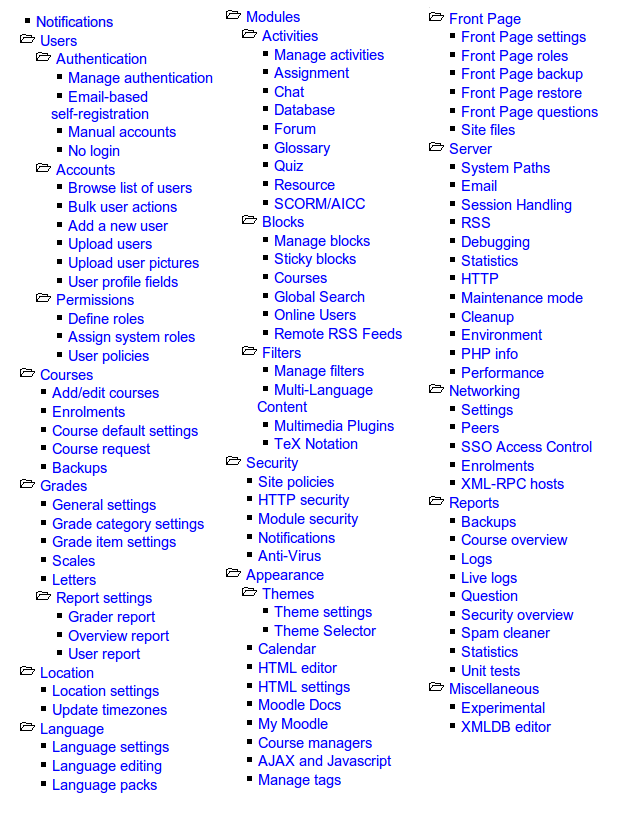
\includegraphics[width=1\linewidth]{images/moodle_panel.png}
  \end{center}
  \caption{Panel administratora w systemie Moodle}
  \label{fig:moodle_panel}
\end{figure}


Moduł do konstruowania i przeprowadzania testów umożliwia tworzenie pytań rodzaju
wielokrotnego lub jednokrotnego wyboru, wyliczeniowych, a nawet otwartych. Minusem tych
ostatnich jest to, że test nie może zostać oceniony automatycznie, punkty muszą zostać
przyznane przez osobę odpowiedzialną za jego przygotowanie. Mając do dyspozycji bank
pytań, możemy przygotować test, decydując o dacie rozpoczęcia, czasie trwania, kolejności
wyświetlanych odpowiedzi, czy ilości podejść. Mnogość opcji konfiguracji sprawia, że
stworzenie nowego rekordu zajmuje dużo czasu, co zdecydowanie obniża motywację podjęcia
takowej próby.


Jako że \emph{Moodle} jest wolnym oprogramowaniem, powstało wiele rozszerzeń
dostarczających nowe możliwości. Między innymi takie jak:

\begin{itemize}
  \item{różnorodne metody uwierzytelnienia}
  \item{motywy graficzne}
  \item{czat}
  \item{kalendarz}
  \item{filtry treści}
  \item{efekty graficzne wykorzystujące JavaScript}
  \item{komunikacja z serwerem za pomocą technologii AJAX}
\end{itemize}


Podsumowując, \emph{Moodle} jest bardzo rozbudowanym systemem. przeznaczonym dla większych
grup. Zawiera w sobie wiele modułów, które są integralnymi elementami całego systemu, dlatego
nie mamy możliwości skupienia się tylko na części do przeprowadzania testów -- musimy
również obsłużyć wszystkie pozostałe funkcje, takie jak forum, tworzenie personalnych
stron, szczegółową konfigurację zarządzania treścią, etc. Powoduje to obciążenie
serwera przez usługi, które de facto nie są używane.

\section{OLAT}
\emph{OLAT}\footnote{OLAT -- Online Learning And Training (ang.)} jest internetowym
systemem zdalnej nauki dostępnym na wolnej licencji. Jest rozwijany od 1999 roku, głównie
na uniwersytecie w Zurychu. Całość została napisana w języku \emph{Java} i do uruchomienia
po stronie klienta wymaga maszyny wirtualnej. Wraz z kolejnymi latami rozwoju, platforma
była wzbogacana o nowe funkcje i obecnie częściami składowymi są między innymi:

\begin{itemize}
  \item{zarządzanie treścią}
  \item{fora}
  \item{testy z różnymi rodzajami pytań}
  \item{wiki}
  \item{ankiety}
  \item{czat}
  \item{moduł oceniania}
  \item{wielojęzyczność}
\end{itemize}


Uruchomienie serwera jest możliwe na większości systemach operacyjnych, wymaganymi
komponentami są:

\begin{itemize}
  \item{Java SDK\footnote{SDK -- Software Development Kit (ang.)}}
  \item{Tomcat Servlet}
  \item{serwer bazy danych, np. MySQL lub PostgreSQL}
\end{itemize}


Wiele znanych uczelni z powodzeniem wdrożyło system \emph{OLAT} do codziennego użytku.
Statystyki na głównej stronie przedstawiają około 150 instalacji na świecie~\cite{olat}.
Pomimo, że główny kod pisany jest w \emph{Javie}, to jednak procentowo, więcej linii kodu
zawierają skrypty \emph{JavaScriptowe}. Służą one do obsługi interfejsu użytkownika,
dlatego też przy wyłączonym interpreterze w przeglądarce, praktycznie żadna funkcja nie
może zostać użyta.


Cała aplikacja jest obszernym narzędziem, przeznaczonym dla większych grup użytkowników.
Podobnie jak w przypadku \emph{Moodle} nie możemy korzystać tylko z modułu
odpowiedzialnego za przeprowadzanie testów. Decydując się na uruchomienie, musimy wziąć
pod uwagę spore zużycie zasobów serwera produkcyjnego.


\cleardoublepage
\chapter{Technologie}
\section{Ruby}
\emph{Ruby} został stworzony w 1995 roku przez Yukihiro Matsumoto, znanego również
pod pseudonimem Matz. Łączy on w sobie cechy kilku języków, między innymi: \emph{Lispa},
\emph{Perla}, \emph{Pythona} czy \emph{Smalltalka}, z każdego wybierając to co najlepsze,
w efekcie dając elastyczne narzędzie, o wielkich możliwościach.\\
Jest to język skryptowy -- aby spróbować jego możliwości wystarczy nam konsolowy
interpreter, z poziomu którego wydajemy polecenia, otrzymując od razu wynik działania.


\emph{Ruby} należy do grupy języków bardzo wysokiego poziomu programowania
(\emph{VHLL})\footnote{VHLL -- Very High-Level Programming Language (ang.)}.
W bibliotece standardowej otrzymujemy szereg metod, dzięki którym bez zbytniego wysiłku,
czasem nawet w jednej linijce, możemy napisać skrypt wykonujący złożone działania.\\
Jedną z głównych cech tego języka, która rzuca się w oczy od razu, jest tzw.
,,samokomentujący się kod''. Składnia jest bardzo zbliżona do języka naturalnego
(angielskiego), dzięki czemu nawet osoba nie mająca nic wspólnego z programowaniem,
powinna przewidzieć co dany kawałek kodu wykonuje. Przykładem niech będzie
listing nr~\ref{listing:selfcommenting}.

\begin{listing}
  \input{listing/selfcommenting}
  \listingcaption{Samokomentujący się kod}
  \label{listing:selfcommenting}
\end{listing}


Ciekawą własnością jest tzw. kacze typowanie\footnote{Duck typing (ang.)}, które polega na
rozpoznaniu typu poprzez zachowanie obiektu a nie jego deklaracji. Przykładowo: jeśli mamy
funkcję przyjmującą argument, to nie musimy określać jakiego on będzie typu, dzięki czemu
możemy wywołać na nim metodę (jeśli takową posiada), odpowiednią dla klasy obiektu. Nazwa
wzięła się z powiedzenia ,,Jeśli chodzi jak kaczka i kwacze jak kaczka, to musi być
kaczką''\footnote{''If it walks like a duck and quacks like a duck, I would call it a duck''
-- James Whitcomb Riley (ang.)}


Kolejną cechą, która jest jedną z najsilniejszych tego języka, jest metaprogramowanie. Nie tyle sama
możliwość, co raczej przystępność i prostota jego użycia. Framework \emph{Ruby on Rails}
korzysta bardzo często z jego dobrodziejstw, dając nam tzw. ,,magię railsów'', czyli
między innymi dynamiczne findery, niemalże bezdeklaratywne asocjacje czy szereg innych
metod, o których więcej w kolejnym podrozdziale.\\
Ogólnie rzecz biorąc język \emph{Ruby} wraz ze swoimi otwartymi klasami stwarza
programiście przestrzeń, w której może się skupić wyłącznie na postawionym problemie, nie
martwiąc się o przeszkody techniczne, takie jak dostęp do modyfikacji metod z zewnętrznych
bibliotek czy rozszerzanie klas o nowe funkcjonalności. Sposób pisania jest intuicyjny,
działa tu zasada najmniejszego zaskoczenia. Często, powstające nowe biblioteki (gemy), trzymają
się kilku ustalonych konwencji, dzięki czemu zgłębiając nowe funkcjonalności, programista
odnajduje duże podobieństwa do już dobrze znanych mu metod, choćby z biblioteki standardowej.


\section{Ruby on Rails}
Twórcą frameworka \emph{Ruby on Rails} jest David Heinemeier Hansson. Powstał on w 2003
roku, obecnie rozwijany cały czas przez społeczność użytkowników i czuwającą nad
spójnością kodu tzw. \emph{Core Team}. Jest wolnym oprogramowaniem\footnote{Open source (ang.)},
stworzonym na licencji \emph{MIT}.\footnote{Licencja powstała w Massachusetts Institute of Technology}\\
Framework jest kompletnym narzędziem do tworzenia aplikacji internetowych z wykorzystaniem
bazy danych. Opiera się na wzorcu projektowym model-widok-kontroler\footnote{MVC -- Model View
Controller (ang.)} i w całości jest napisany w języku \emph{Ruby}.


Główną zasadą jaką kierują się twórcy, to tzw. konwencja nad
konfiguracją\footnote{Convention over Configuration (ang.)}, dzięki której przy minimalnej
ilości kodu, dostajemy ogromną funkcjonalność, co znacznie przyspiesza tworzenie
aplikacji. Świetnym przykładem jest \emph{screencast}, na którym Ryan
Bates\footnote{Ryan Bates -- jeden z aktywistów Ruby on Rails, znany głównie jako autor
darmowych, cotygodniowych screencastów \cite{ryan-bates}} tworzy w 15 minut szkielet
systemu blogowego, uwzględniając takie dodatki jak dostępność poprzez kanał
RSS\footnote{RSS -- Really Simple Syndication (ang.)} czy reprezentacja zasobów w postaci
\emph{XML} \cite{blog-in-15-min}.\\
Kolejną zaletą takiego podejścia, jest przejrzystość kodu. Dopóki postępujemy zgodnie ze
wskazówkami, nasz kod nie powinien być trudny do zrozumienia przez innego programistę,
również zajmującego się tą technologią.\\
Drugą ideą składającą się na całość tzw. \emph{Rails way} jest zapobieganie powtarzaniu
samego siebie\footnote{DRY -- Don't Repeat Yourself (ang.)}. Jeśli w jakimś miejscu używamy
tego samego fragmentu kodu (czasem wręcz przeklejonego), to znaczy że możemy to zrobić
prościej. Pomoc przychodzi z samego języka \emph{Ruby}, w którym za pomocą mechanizmu
tzw. \emph{Mixinów}, możemy dodawać do interesujących nas klas czy modułów gotowe zestawy
metod, upraszczając w ten sposób strukturę kodu.


Po wygenerowaniu szkieletu projektu, dostajemy drzewo katalogów, które między innymi
odzwierciedlają wykorzystanie wzorca \emph{MVC}. Pliki odpowiedzialne za interakcję z
bazą danych oraz główną logikę aplikacji znajdują się w katalogu \texttt{models}. Część
z wygenerowanymi widokami, czyli dokumentami \emph{HTML} również ma swoje określone miejsce w
katalogu \texttt{views}, natomiast część obsługująca akcje użytkownika przesyłane do serwera
oraz łącząca ze sobą poprzednio wymienione komponenty, można znaleźć w
katalogu \texttt{controllers}. Wszystko to zapewnia odpowiednią separację kodu, dzięki
czemu modyfikacje poszczególnych elementów nie powinny wpływać na siebie.


\subsection{Gemy}
\emph{Ruby on Rails} składa się z kilku odrębnych \texttt{gemów}\footnote{Gemy -- system
paczek, bibliotek dostarczający nową funkcjonalność}, które mogą być również używane
osobno, poza frameworkiem (nie posiadają zależności między sobą). Są to:

\begin{itemize}
  \item{ActionMailer}
  \item{ActionPack}
  \item{ActiveRecord}
  \item{ActiveResource}
  \item{ActiveSupport}
\end{itemize}


\emph{ActionMailer} odpowiada za obsługę usług pocztowych wychodzących i przychodzących z
naszej aplikacji. Jako generator widoków może być używany \emph{ERb}\footnote{ERb --
Embedded Ruby (ang.) -- system szablonów umożliwiający zagnieżdżanie kodu Rubiego w
dokumencie tekstowym}. Konfiguracja jest możliwa dla każdego środowiska -- odpowiednio w
środowisku produkcyjnym wpisuje się dane rzeczywiste serwera pocztowego,
natomiast w deweloperskim oraz testowym, można zastąpić ją wersją próbną, która nie
będzie próbowała się łączyć z serwerem pocztowym, natomiast cały mechanizm i logika
zostaną zachowane.


\emph{ActionPack} obsługuje kontrolery oraz widoki. Przychodzące
zapytanie z serwera jest wiązane z odpowiednią akcją kontrolera za pomocą tzw.
\emph{Routingu}, który mapuje ścieżkę adresu na parametry przekazywane do aplikacji.
Obecnie domyślny i preferowany sposób konstruowania ścieżek \emph{URL} jest zgodny z
\emph{REST}.\footnote{REST -- Representational State Transfer (ang.) -- reprezentacja zasobu
poprzez ,,czasowniki'' protokołu HTTP: GET, POST, PUT, DELETE (więcej na stronie~\pageref{sec:rest})}\\
Wywołana akcja musi zwrócić odpowiedź, bądź to w postaci wyrenderowanego widoku,
przekierowania czy też kodu błędu zgodnego z protokołem \emph{HTTP}. Ciekawym mechanizmem,
którym dysponuje moduł \emph{ActionController} są filtry. Pozwalają one na wyzwolenie
logiki przed lub po odwołaniu się do docelowej akcji. Często wykorzystywane są przy
uwierzytelnieniu, aby zabezpieczyć treść strony przed niepowołanymi osobami. W tym
miejscu mamy też dostęp do ,,ciasteczek''\footnote{Cookies (ang.) -- niewielkie informacje
tekstowe przechowywane po stronie klienta} i sesji (rozwiązanie problemu bezstanowości
protokołu \emph{HTTP}). W \emph{Ruby on Rails} sesja jest niczym innym jak tablicą
asocjacyjną, do której możemy się odwoływać za pomocą kluczy. Sposób
przechowywania sesji pomiędzy kolejnymi żądaniami jest konfigurowalny. Może ona być
zapisywana zarówno w bazie danych jak i w ciasteczku.\\
Najczęściej po wykonaniu akcji jest renderowany widok, zgodnie z konwencją jest to plik o
tej samej nazwie co akcja, znajdujący się w katalogu \texttt{views} i podkatalogu
odpowiadającemu nazwie kontrolera (oczywiście jest możliwe przekazanie nazwy eksplicite).
Rozszerzenie pliku składa się z nazwy żądanego formatu (html, js, xml, etc.) oraz systemu
szablonów, który ma zostać użyty (erb, haml, builder, etc.) np. \texttt{index.html.haml}.


\emph{ActiveRecord} działa jako domyślne mapowanie
obiektowo-relacyjne\footnote{ORM -- Object-Relational Mapping (ang.)},
czyli odwzorowanie logiki powiązanych ze sobą modeli na bazę danych.
Nazwa została wzięta z książki Martina Fowlera \cite{martin-fowler}, która
właśnie opisuje powyższe zagadnienie. Moduł ten nie jest ściśle związany z żadną
wersją bazy danych i może być z powodzeniem używany z \emph{SQLite},
\emph{MySQL}, \emph{PostgreSQL} czy \emph{Oracle}. Pozwala między innymi na
konstruowanie zapytań za pomocą kodu \emph{Rubiego}, który później jest
przekształcany na odpowiadającą mu składnię \emph{SQLa}.
Przykład przedstawiony na listingu nr~\ref{listing:activerecord-finders}.

\begin{listing}
  \input{listing/activerecord_finders}
  \listingcaption{Konstruowanie zapytań oraz wygenerowany kod SQL}
  \label{listing:activerecord-finders}
\end{listing}


Jak można zauważyć, w prosty sposób konstruuje się zapytania, nie dotykając w ogóle
czystego \emph{SQLa}. Drugi i trzeci przykład wygenerowały to samo zapytanie.
Składnia tego ostatniego jest przyjemniejsza dla oka, a umożliwiają nam je tzw.
dynamiczne findery, które za pomocą metaprogramowania są tworzone w ,,locie''.
Jest to cecha języka \emph{Ruby}. Możemy przechwycić wywołanie nieistniejącej
metody na obiekcie, poprzez przedefiniowanie funkcji \emph{method\_missing},
która jako argumenty przyjmuje kolejno: symbol wywołanej metody, oraz wszystkie
pozostałe argumenty przekazane do niej. W powyższym przykładzie symbol
\emph{:find\_by\_login} jest parsowany do słów \emph{find\_by} oraz \emph{login}, który
następnie próbuje zostać odnaleziony jako kolumna w tabeli odpowiadającej klasie
\emph{User}. Jeśli to się powiedzie, konstruowane jest zapytanie \emph{SQL}
wykorzystujące argument \emph{johndoe} jako parametr wywołania.\\
Kolejnym elementem stworzonym za pomocą metaprogramowania są asocjacje. Powiązanie
dwóch obiektów sprowadza się do jednej linijki kodu w ciele klasy, jak na
listingu nr~\ref{listing:activerecord-association}.

\begin{listing}
  \input{listing/activerecord_association}
  \listingcaption{Powiązanie dwóch obiektów ActiveRecord}
  \label{listing:activerecord-association}
\end{listing}


Jeśli trzymamy się konwencji, to powyższy zapis jest wystarczający, musimy tylko
pamiętać o umieszczeniu kolumny \texttt{student\_id} w tabeli \texttt{exams}. Jak
widzimy konstrukcja odpowiada naturalnej relacji w języku angielskim, dlatego
też nie powinno się używać lokalizowanych nazw tabel, co zapewnia spójność i
nie powoduje ,,potworków językowych'', takich jak \texttt{student has many
egzamins}. Po deklaracji asocjacji dostajemy automatycznie między innymi takie
metody jak przedstawione na listingu nr~\ref{listing:activerecord-association-finders}.

\begin{listing}
  \input{listing/activerecord_association_finders}
  \listingcaption{Dostępne metody po deklaracji asocjacji}
  \label{listing:activerecord-association-finders}
\end{listing}


Walidatory zapewniają poprawność wprowadzanych danych, dzięki którym można
również poinformować użytkownika o rodzaju błędu. Mamy do dyspozycji szereg
standardowych metod, najczęściej używanych, ale również możemy tworzyć swoje
własne. Przykładowy sposób użycia przedstawia listing
nr~\ref{listing:activerecord-validations}.

\begin{listing}
  \input{listing/activerecord_validations}
  \listingcaption{Walidacja danych}
  \label{listing:activerecord-validations}
\end{listing}


W podanym przykładzie pierwsza walidacja zapewnia nam obecność nazwy egzaminu,
druga sprawdza czy czas trwania (\texttt{duration}) jest liczbą całkowitą, większą od
zera. Ostatni walidator jest metodą zdefiniowaną przez programistę i jest on
wywoływany jedynie gdy wartość pola ,,ilość pytań'' (\texttt{question\_number}) nie jest pusta.
Zapewnia, że liczba ta nie może być większa niż ilość wszystkich dostępnych
pytań dla danego egzaminu. Symbol dodawanego błędu możemy następnie zlokalizować
w plikach z tłumaczeniami.


Kolejną przydatną rzeczą są wywołania zwrotne -- pozwalają na manipulację
atrybutami, przed lub po walidacji, utworzeniu, uaktualnieniu lub usunięciu
obiektu z bazy danych. Dzięki temu możemy w dokładnie określonym momencie
wyzwolić odpowiednią logikę. Wywołania działają również przy deklarowanej
asocjacji, więc dodatkowo dostajemy możliwość wywołania metod przy dodawaniu i
usuwaniu powiązanych obiektów. Przykładowe \texttt{callbacki} znajdują się na listingu
nr~\ref{listing:activerecord-callbacks}.

\begin{listing}
  \input{listing/activerecord_callbacks}
  \listingcaption{Wywołania zwrotne}
  \label{listing:activerecord-callbacks}
\end{listing}


Operowanie atrybutami w podany sposób jest bardzo wygodne, szczególnie że jest
zapewniona atomowość modelu. Jeśli powiązane modele również są modyfikowane, to
w chwili np. błędu walidacji, lub innego niepowodzenia, wszystkie zmiany są
cofane do stanu pierwotnego. Innymi słowy, zmiany są wprowadzane do obiektów
tylko jeśli wszystko jest przeprowadzone pomyślnie. Z transakcji możemy również
korzystać jawnie, przekazując do metody \texttt{transaction} blok, w którym
wykonujemy interesujące nas akcje.


Zmian schematu bazy danych dokonujemy poprzez migracje. Są to pliki z kodem \emph{Rubiego},
w których definiujemy wprowadzane tabele oraz poszczególne kolumny. Świetnie sprawdzają
się przy pracy w zespole, gdyż każdy plik jest oznaczony datą, a sama baza danych
przechowuje informację o aktualnej wersji, dlatego nie ma tu konfliktów i nie musimy
przejmować się kolejnością wprowadzanych zmian. Mamy do dyspozycji kilka generatorów,
które znacznie ułatwiają i przyspieszają pracę. Dodatkowo bazują one na konwencji -- nazwa
modelu (klasy) w liczbie pojedynczej, natomiast nazwa kolumny w liczbie mnogiej, co
minimalizuje możliwość popełnienia błędu przez programistę. Przykładowe polecenie oraz
wygenerowany plik znajduje się na listingu nr~\ref{listing:activerecord-migrations}.

\begin{listing}
  \input{listing/activerecord_migrations}
  \listingcaption{Generator modelu oraz automatycznie utworzony plik migracji}
  \label{listing:activerecord-migrations}
\end{listing}


Ostatecznie zmiany wprowadzamy poprzez polecenie \texttt{rake db:migrate}\footnote{Rake --
Ruby Make -- odpowiednik uniksowego Make, pozwalający na użycie języka Ruby. Twórcą
jest Jim Weirich}. Domyślnie \texttt{railsy} dodają dwie tzw. magiczne kolumny
\texttt{created\_at} oraz \texttt{updated\_at}, które są aktualizowane automatycznie, jak
nie trudno się domyślić przy utworzeniu obiektu oraz jego aktualizacji.


\emph{ActiveResource} jest biblioteką umożliwiającą komunikację z innymi
aplikacjami railsowymi niemal przy tej samej składni jaka jest dostępna w \emph
{ActiveRecord}. Wystarczy że określimy \emph{host} zdalnego serwera i już
możemy korzystać z jego \emph{API},\footnote{API -- Application Programming
Interface (ang.) -- tutaj interfejs do komunikacji ze zdalną aplikacją} o ile
jest zgodne z konwencją REST\footnote{więcej na stronie~\pageref{sec:rest}}.
Moduł jest oparty o prezentację zasobów w postaci \emph{XML} lub
\emph{JSON}\footnote{JSON -- JavaScript Object Notation -- tekstowy format wymiany
danych, będący podzbiorem języka JavaScript}.


\emph{ActiveResource} przynosi między innymi rozszerzenia biblioteki
standardowej o nowe metody, ułatwiające konwersję lub kalkulację na podstawowych
typach, takich jak \texttt{String}, \texttt{Date} czy \texttt{Numeric}. Przykłady
wykorzystania zostały przedstawione na listingu nr~\ref{listing:activesupport}.

\begin{listing}
  \input{listing/activesupport}
  \listingcaption{Przykład dostępnych metod w ActiveSupport}
  \label{listing:activesupport}
\end{listing}


W ostatnim przykładzie widzimy metodę z pytajnikiem. Warto wspomnieć w tym
momencie o konwencji jaka przyjęła się w środowisku języka \emph{Ruby}, gdzie
właśnie metody zakończone pytajnikiem zwracają zawsze \texttt{true} lub
\texttt{false}, natomiast kończące się wykrzyknikiem są ,,groźniejszą'' wersją metody
bez wykrzyknika, co na przykład może oznaczać trwałą modyfikację obiektu.

\subsection{Internacjonalizacja}
Poczynając od wersji 2.2, \emph{Ruby on Rails} ma wbudowany mechanizm internacjonalizacji.
Tłumaczenie słów w widokach odbywa się poprzez wywołanie metody \texttt{translate}
aliasowanej do \texttt{t()} na słowie, które de facto jest kluczem. Następnie w plikach z
tłumaczeniem owemu kluczowi jest przypisywana konkretna, lokalizowana wartość.
Dodatkowo możemy tłumaczyć nazwy modeli i atrybutów oraz błędy
walidacji. Pliki z tłumaczeniem mogą być z rozszerzeniem \texttt{.rb}, wtedy zapisujemy je
w postaci tablic asocjacyjnych języka \emph{Ruby} lub z rozszerzeniem \texttt{.yml}.
\emph{YAML}\footnote{YAML -- YAML Ain't Markup Language (ang.)} jest językiem formalnym
przeznaczonym do reprezentowania zbioru danych. Jego główną zaletą jest czytelność,
przeciwnie jak to jest w przypadku \emph{XMLa}. Nie ma tu otwieranych i zamykanych
znaczników, gdyż struktura bazuje na wcięciach, określając tym samym poziom zagnieżdżenia.


\subsection{Bezpieczeństwo aplikacji}
\emph{Ruby on Rails} ma wbudowane mechanizmy oraz metody pomagające zabezpieczyć się
przed najbardziej znanymi próbami ataku na naszą aplikację. Jednym z nich jest
\emph{CSRF}\footnote{CSRF -- Cross-site request forgery (ang.)}, który polega na podszyciu się
napastnika pod sesję użytkownika. Jeśli osoba taka jest zalogowana, wystarczy że uruchomi
odnośnik modyfikujący dane niedostępne bez aktywnej sesji. Innymi słowy, zmusza się
użytkownika do wysłania żądania \emph{HTTP} do serwera z jego przeglądarki, wykorzystując
jego uwierzytelnienie.\\
Sposobem na przeciwdziałanie jest dołączanie do parametrów przesyłanych do serwera,
unikalnego tokena, który jednoznacznie identyfikuje użytkownika. Token ten jest umieszczany
automatycznie w formularzach, gdzie wysyłamy żądania metodą \emph{POST}. Następnie po
stronie serwera jest porównywany z aktualnym kluczem sesji użytkownika. Dzięki temu
eliminujemy spreparowane formularze, które próbują modyfikować poufne dane.\\
Domyślnie mechanizm ten jest włączony dla każdej nowo tworzonej aplikacji railsowej i
sprowadza się do umieszczenia w kontrolerze głównym linijki: \texttt{protect\_from\_forgery}.


Kolejnym sposobem ataku może być tzw. \emph{XSS}\footnote{XSS -- Cross-site scripting
(ang.)} polegający na osadzeniu, w treści kodu strony, skryptu (najczęściej
javascriptowego), który może wydobyć z bazy danych poufne informacje. Przykładem niech
będzie serwis, na którym każdy użytkownik może pozostawić komentarz. Jeśli nie jest on
zabezpieczony, możemy wkleić kod, który przy kolejnym wyświetleniu strony, będzie potraktowany
przez naszą aplikację jako regularny kawałek kodu aplikacji, a więc zostanie wykonany.\\
Z pomocą przychodzi metoda \texttt{html\_escape} aliasowana jako po prostu \texttt{h()},
która zawsze traktuje przekazane słowa jako czysty tekst, lub metoda \texttt{sanitize},
dopuszczająca pewne zdefiniowane tagi \emph{HTMLowe}, które są uznawane za ,,bezpieczne''.


\subsection{Wdrażanie aplikacji}
Wdrażanie wersji produkcyjnej dotyczy serwera \emph{HTTP} oraz bazy danych, gdzie musimy
wziąć pod uwagę wydajność i szybkość obsłużenia zapytania. W wersji rozwojowej
wystarczające są domyślnie używane narzędzia, czyli napisany w \emph{Rubim} \emph{Webrick},
który służy nam jako lokalny serwer \emph{HTTP} oraz \emph{SQLite} jako system
zarządzania bazą danych.


\emph{SQLite} świetnie sprawdza się przy rozwoju aplikacji, gdyż baza danych jest trzymana
w jednym pliku umieszczonym w dogodnym dla nas miejscu. Nie musimy się przejmować
rozporządzaniem prawami dostępu czy zarządzaniem użytkownikami, a jeśli potrzebujemy nagle
usunąć istniejącą bazę, sprowadza się to po prostu do usunięcia danego pliku.
Co ciekawe \emph{SQLite} wydajnościowo wypada bardzo dobrze w przypadku jednego
użytkownika, dlatego jest używany w systemach wbudowanych\footnote{Embedded system (ang.) --
system komputerowy specjalnego przeznaczenia, który staje się integralną częścią
obsługiwanego przez niego sprzętu \cite{embedded-system}} takich jak telefony komórkowe
czy urządzenia \emph{AGD}. Jednak przy obsłudze strony internetowej, gdzie jednoczesnych zapytań
skierowanych do bazy danych może być dużo, jest potrzebny osobny serwer. Jednym
z najczęściej spotykanych wyborów jest \emph{PostgreSQL} lub \emph{MySQL}. Konfiguracja
po stronie railsów wymaga jedynie określenia nazwy użytkownika i ewentualnego hasła, które
zapisujemy w pliku \texttt{config/database.yml}.


Początkowo produkcyjnymi serwerami \emph{HTTP} były \emph{Mongrel} i \emph{Thin}, które
częściowo były pisane w języku \emph{C}, jednak od czasu wydania \emph{Phusion Passengera},
znanego również jako \texttt{mod\_rails} lub \texttt{mod\_rack}, rekomendowanym i
jednocześnie najczęściej używanym jest serwer \emph{Apache}.


\emph{Phusion Passenger} jest modułem, dostępnym jako \texttt{gem}, który umożliwia
uruchomienie aplikacji pisanych w języku \emph{Ruby} opartych o bibliotekę \emph{Rack} na
serwerze \emph{HTTP} \emph{Apache}. \emph{Rack} z kolei, również w postaci \texttt{gema},
dostarcza uniwersalny interfejs do naszego kodu, dzięki któremu wszelkie serwery
wspierające \emph{Rubiego} mogą go hostować.


\subsection{Merb + Ruby on Rails}
\emph{Merb} początkowo był małym frameworkiem napisanym w języku \emph{Ruby}, aby w
przeciągu kilku lat rozwinąć się i konkurować ze swoim starszym bratem \emph{Ruby on
Rails}. Twórcą jest Ezra Zygmuntowicz, który skupił się na szybkości działania aplikacji
oraz uniezależnieniu frameworka od konkretnej biblioteki \emph{ORM} oraz \emph{JavaScript}.
\emph{Merb} nastawiony był również na większą modularność, sam w sobie nie dawał tak
dużej funkcjonalności jak \emph{RoR}, ale rozszerzenie o nowe możliwości miało być
prostsze i wspierane przez zespół pracowników czuwających nad głównym kodem.\\
W dniu 23 grudnia 2008 roku została ogłoszona wiadomość \cite{rails-merb} o połączeniu obu zespołów,
które razem skupią się na przeniesieniu najlepszych rzeczy z obu frameworków do jednego,
wypuszczonego pod nazwą \emph{Ruby~on~Rails~3.0}. Pierwszej wersji możemy się spodziewać
pod koniec 2009 roku. Informacja ta wzbudziła wiele emocji w środowisku deweloperskim, co
oczywiście przeniosło się też na promocję samych railsów. Obecnie, framework ten jest
jednym z najpopularniejszych i większość startujących, głównie opensourcowych,
projektów wybiera właśnie \emph{Ruby on Rails}.\\
Spodziewane zmiany wraz z wydaniem wersji 3.0 to przede wszystkim większa
wydajność oraz niezależność. Będzie możliwy swobodny wybór bibliotek odpowiedzialnych za
\emph{JavaScript}, \emph{ORM}, silnik szablonów oraz moduł testujący. Twórcy zapewniają
również, że migracja aplikacji pisanych we wcześniejszych wersjach oraz \emph{Merbie} do nowej
wersji, nie będzie stwarzać problemu.


\section{REST}\label{sec:rest}
\emph{REST}\footnote{REST -- Representational State Transfer (ang.)} jest wzorcem
architektury oprogramowania, który próbuje przedstawić reprezentację zasobów oraz
zarządzanie nimi poprzez odpowiednie metody protokołu \emph{HTTP}. Możemy zobrazować to w
następujący sposób: adres \emph{URI} jest identyfikatorem określającym konkretny zasób
(obiekt), możemy myśleć o nim jako o rzeczowniku. Dopełnieniem sentencji jest czasownik,
który jest przedstawiony jako jedna z metod protokołu \emph{HTTP}: \emph{POST}, \emph{GET},
\emph{PUT} lub \emph{DELETE}. Budujemy gramatycznie poprawne ,,zdanie'' poprzez
połączenie rzeczownika z czasownikiem, otrzymując formę wywołania przesyłaną na serwer dla
konkretnego zasobu. Odpowiednio, chcąc pobrać dane, bez modyfikacji, powinniśmy użyć
metody \emph{GET}. \emph{POST} służy do tworzenia nowych obiektów, \emph{PUT} do ich
modyfikacji, natomiast \emph{DELETE} do usuwania.\\
Łączy się to wszystko świetnie z wykorzystaniem \emph{CRUD}\footnote{CRUD -- create, read,
update and delete (ang.)}, który sprowadza się do podstawowych akcji wykonywanych na
obiektach połączonych z bazą danych. Zestawienie przedstawia tabela nr \ref{table:rest}.

\begin{table}[htcb]
  \begin{center}
    \begin{tabular}{|c|c|c|c|}
      \hline
      \textbf{metoda HTTP} & \textbf{CRUD} & \textbf{SQL} & \textbf{akcja RoR}\\
      \hline
      \texttt{POST} & \texttt{Create} & \texttt{Insert} & \texttt{create}\\
      \texttt{GET} & \texttt{Read} & \texttt{Select} & \texttt{show}\\
      \texttt{PUT} & \texttt{Update} & \texttt{Update} & \texttt{update}\\
      \texttt{DELETE} & \texttt{Delete} & \texttt{Delete} & \texttt{destroy}\\
      \hline
    \end{tabular}
  \end{center}
  \caption{Powiązanie REST, CRUD, zapytań SQL oraz akcji RoR}
  \label{table:rest}
\end{table}

Jeśli trzymamy się przyjętych konwencji, to przykładowy ciąg zdarzeń dla usunięcia danego
obiektu np. użytkownika, wyglądałby następująco: na serwer jest przesyłane żądanie pod
adresem \texttt{users/1}, gdzie \texttt{1} jest identyfikatorem osobnika, którego chcemy
usunąć z bazy danych. Żądanie jest przesyłane metodą \emph{DELETE}, następnie po stronie
aplikacji mapowane na akcję \texttt{destroy} w kontrolerze \emph{UsersController},
aż w końcu przy użyciu \emph{ActiveRecord} jest generowane zapytanie \emph{SQL}, które
ostatecznie usuwa obiekt z bazy.\\
Warto wspomnieć w tym momencie, że przeglądarki obecnie nie wspierają wysyłania żądań
\emph{PUT} oraz \emph{DELETE}, co jednak railsy załatwiają poprzez dodanie do
formularza ukrytego pola z nazwą docelowej metody, używając żądania \emph{POST}.\\
Domyślnym sposobem budowania aplikacji w \emph{Ruby on Rails} poczynając od wersji 2.0
jest właśnie \emph{REST}, który ma też duże znaczenie w przypadku wykorzystania \emph{ActiveResource},
czyli budowania \emph{API} w celu udostępnienia zasobów dla innych
serwisów. Sprowadza się to praktycznie tylko do przedstawienia konkretnego obiektu lub
kolekcji poprzez format \emph{XML} lub \emph{JSON}.


\section{Testy jednostkowe}
\emph{Shoulda} jest biblioteką służącą do przeprowadzania testów jednostkowych w oparciu o
\emph{BDD}\footnote{BDD -- Behaviour Driven Development (ang.)}. Ideą takiego podejścia
jest pisanie testów jeszcze przed stworzeniem kodu aplikacji, który opisuje funkcjonalność
jakiej mamy się spodziewać. Następnie piszemy kod właściwy, w taki sposób aby test
zakończył się powodzeniem. Później możemy zająć się refaktoryzacją, zabezpieczając się
cały czas istniejącymi testami, przed ewentualnym naruszeniem integralności kodu całej
aplikacji. Testy jednostkowe powinny zapewnić poprawne działanie tworzonych metod w
obrębie tylko jednej klasy. Jeśli jednak istnieją powiązania z innymi modelami, powinniśmy
się zastanowić nad użyciem jednej z bibliotek \emph{mockowania}\footnote{mock -- symulacja
zachowania prawdziwych obiektów w celach testowych}.\\
\emph{Shoulda} jest rozszerzeniem standardowej biblioteki testującej języka \emph{Ruby}
\emph{Test::Unit}, która dostarcza wygodniejszą składnię oraz nowe typy asercji.
Przykładowy test znajduje się na listingu nr~\ref{listing:shoulda}.

\begin{listing}
  \input{listing/shoulda}
  \listingcaption{Przykład testu jednostkowego}
  \label{listing:shoulda}
\end{listing}


Testowane jest przejście stanu egzaminu (implementowanego za pomocą maszyny stanowej,
więcej na stronie nr~\pageref{sec:state_machine}) w rozpoczęty, po którym powinna być
zachowana w bazie danych data i czas. W metodzie \texttt{setup}, która przygotowuje
dostępne obiekty w obrębie danego kontekstu dla każdego testu jednostkowego, przykładowy
rekord został utworzony za pomocą gema \texttt{factory\_girl}. Zastępuje on domyślny
system tworzenia railsowych obiektów testowych, wczytywanych z plików \emph{YAML}, na
rzecz dynamicznie tworzonych obiektów w ciele testu.

\section{Testy integracyjne}
\emph{Cucumber}\footnote{Stworzony w języku Ruby przez Aslaka Hellesøya, więcej na stronie
internetowej \cite{cucumber}} zalicza się do tzw. \emph{Scenario Driven Development} i
służy do testowania funkcjonalności ostatecznej -- tej widocznej dla użytkownika. Polega
na napisaniu scenariusza, który zawiera poszczególne akcje użytkownika wykonywane z
poziomu przeglądarki. Składnia ogranicza się do kilku słów kluczowych, które poprzedzają
dowolny tekst opisujący zdarzenia. Następnie za pomocą wyrażeń regularnych tekst jest
mapowany na definicję metod, pisanych już w języku \emph {Ruby}. Przykład można zobaczyć
na listingu nr~\ref{listing:cucumber}.

\begin{listing}
  \input{listing/cucumber}
  \listingcaption{Przykład testu integracyjnego}
  \label{listing:cucumber}
\end{listing}


Każda linijka jest osobnym krokiem, które są definiowane w plikach pomocniczych.
Przykładową implementację kroków przedstawia listing nr~\ref{listing:cucumber-steps}.

\begin{listing}
  \input{listing/cucumber_steps}
  \listingcaption{Implementacja kroków użytych w scenariuszu}
  \label{listing:cucumber-steps}
\end{listing}


Za pomocą wyrażeń regularnych odnajdywane są przekazane w danym kroku parametry, które
posłużą do wygenerowania odpowiedniej treści. Do poruszania się po stronie w
wirtualnej przeglądarce jest użyty gem \emph{Webrat}, który parsując dokument
\emph{HTML} uzupełnia odpowiednie pola o przekazane atrybuty, a następnie symuluje
komunikację z serwerem przyjmując jego rzekomą odpowiedź.

\section{Haml i Sass}
\emph{Haml}\footnote{Haml -- HTML Abstraction Markup Language (ang.)} jest językiem
znaczników, który opisuje \emph{HTML} i \emph{XHTML}. Składnia wykorzystuje wcięcia, tak więc podobnie
jak w języku \emph{Python} nie musimy domykać raz otwartych tagów. Dzięki temu struktura
szablonu jest bardziej przejrzysta i trudniej jest się pomylić, gdyż przy błędnej składni
zostanie zwrócony wyjątek. Jak wiadomo, w przypadku \emph{HTMLa}, nawet jeśli zapomni się
domknąć tag, to dokument i tak będzie wyświetlony w przeglądarce, błędy nie zwracają
wyjątku.\\
\emph{Haml} nie jest ściśle związany z żadnym językiem programowania i może być używany
również we frameworkach opartych o \emph{Python}, \emph{PHP} czy \emph{.NET}, co czyni
z niego narzędzie warte uwagi dla każdego dewelopera.


\emph{Sass}\footnote{Sass -- Syntactically Awesome Stylesheets (ang.)} jest dostępny razem
z biblioteką \emph{Haml} i służy do generowania kaskadowych arkuszy stylów (\emph{CSS
}\footnote{CSS -- Cascading Style Sheets (ang.)}). Również bazuje na wcięciach, więc
wszelkie tagi są domykane automatycznie. Dodatkową zaletą poza przejrzystością i
zwięzłością języka, jest dostępność zmiennych, na których możemy wykonywać operacje
matematyczne. Przykładowo, jeśli mamy zdefiniowany jeden kolor i chcemy uzyskać np.
jaśniejszy, wystarczy że odejmiemy odpowiednią liczbę od głównego. Kolejną cechą jest
obecność tzw. \texttt{mixinów}, dzięki którym można używać jednego fragmentu kodu w wielu
miejscach, bez powtarzania. Przykład znajduje się na listingu nr~\ref{listing:sass}.

\begin{listing}
  \input{listing/sass}
  \listingcaption{Szablon w języku Sass generujący CSS}
  \label{listing:sass}
\end{listing}


\section{Blueprint i Compass}\label{sec:compass}
\emph{Blueprint} jest frameworkiem \emph{CSS}, który posiada wiele gotowych arkuszy stylów
dotyczących poszczególnych sekcji strony internetowej, takich jak formularze, typografia,
listy, tabele, etc. Używamy go poprzez dołączenie odpowiednich klas lub identyfikatorów do
znaczników \emph{HTMLa}. Zyskujemy automatyczne stylowanie, które oparte jest na
najlepszych doświadczeniach deweloperskich.\\
\emph{Blueprint} stara się ustandaryzować podział strony na najczęściej spotykane sekcje,
takie jak nagłówek, nawigacja, treść, stopka, które mają mieć swoje odpowiednie
znaczniki w przygotowywanej 5 wersji języka \emph{HTML}. Ciekawym pomysłem jest
stylowanie względem siatki, która rozdziela stronę na kilkanaście pasów. Wszelkie marginesy
oraz przesunięte elementy są dostosowywane do rozmiarów tychże części, dzięki czemu
estetyka strony jest zachowana.


\emph{Compass}\footnote{Twórcą jest Chris Eppstein, więcej na stronie internetowej
\cite{compass}} jest narzędziem napisanym w języku \emph{Ruby}, wykorzystującym język
\emph{Sass} oraz łączącym kilka najpopularniejszych frameworków \emph{CSS}, w tym
\emph{Blueprinta}. Jego główną cechą jest to, że nie trzeba dodawać określonych klas i
identyfikatorów do znaczników \emph{HTMLa}, aby korzystać z dobrodziejstw gotowych stylów.
To programista podporządkowuje zebrane arkusze pod strukturę strony. Głównie za sprawą
dostępnych w \emph{Sassie} \texttt{mixinów} jest możliwe dodawanie pojedynczych
fragmentów gotowych rozwiązań.\\
Automatycznie dostajemy również wersję arkuszy stylów do druku strony i dla przeglądarki \emph{Internet
Explorer}, która niestety nie trzyma się przyjętych przez \emph{W3C}\footnote{W3C -- The
World Wide Web Consortium (ang.) -- organizacja zajmująca się ustanawianiem standardów pisania i
przesyłu stron WWW} standardów i często trzeba korygować jej niedoskonałości. Dotyczy to
zwłaszcza starszych wersji przeglądarek \emph{IE}, które na szczęście wychodzą powoli z
użytku.


\section{jQuery}
\emph{jQuery} jest biblioteką napisaną w \emph{JavaScripcie}, która dostarcza szereg
gotowych rozwiązań, najczęściej spotykanych na stronach internetowych. Duży wpływ na
rozwój kodu, oprócz twórcy Johna Resiga, ma Yehuda Katz, zajmujący się również rozwojem
\emph{Merba} oraz \emph{Ruby on Rails} (od czasu połączenia obu frameworków).
Jedną z głównych zalet jest niezależność od przeglądarki. Dostępne \emph{API} jest
uniwersalne, a więc biblioteka sama dba o wyrównanie nieścisłości wynikających właśnie ze
środowiska działania.\\
Dzięki \emph{jQuery} w prosty sposób możemy manipulować modelem \emph{DOM}\footnote{DOM --
Document Object Model (ang.)}, wykorzystując wygodne w użyciu selektory. Kolejną dostępną
funkcjonalnością jest komunikacja z serwerem za pomocą technologii
\emph{AJAX}\footnote{AJAX -- Asynchronous JavaScript and XML (ang.)}, która sprowadza się
jedynie do wywołania odpowiedniej funkcji. Tworzenie własnych rozszerzeń nie sprawia
problemu, dzięki czemu ilość dostępnych dodatków jest ogromna.

\section{Git}
\emph{Git} jest rozproszonym systemem kontroli wersji stworzonym przez Linus Torvaldsa w 2005 roku.
Został on napisany na potrzeby rozwoju jądra \emph{Linux}, jednak obecnie jest używany
przez wiele znanych projektów, choćby takich jak: \emph{Android}, \emph{Amarok}, \emph{Perl},
czy \emph{Ruby on Rails}. Głównym celem była szybkość działania oraz nie powtarzanie błędów
zaistniałych w \emph{CVS}\footnote{CVS -- Concurrent Versions System (ang.)}.
Każdy katalog roboczy jest kompletnym repozytorium, które nie jest uzależnione od dostępu
do sieci czy centralnego serwera, co sprawia że świetnie sprawdza się również przy projekcie
prowadzonym tylko przez jedną osobę.\\
Jedną z możliwości hostowania repozytoriów oferuje \emph{GitHub} \cite{github}, który jest
skupiskiem wielu opensourcowych projektów. Statystyki na dzień 27.07.2009 mówią o 90.000
unikalnych publicznych repozytoriach znajdujących się na serwerach firmy \cite{github-statistics}.


\cleardoublepage
\chapter{Opis środowiska uruchomienia}
\section{Ubuntu}
Aby uruchomić aplikację na systemie \emph{Ubuntu} wymagane są:
\begin{itemize}
  \item{Ruby wraz z interpreterem}
  \item{System paczek RubyGems}
  \item{Odpowiednie gemy (m.in. rails)}
  \item{Biblioteka imagemagick do obróbki ilustracji}
  \item{Biblioteka obsługująca bazę danych formatu SQLite3}
\end{itemize}


Opisany poniżej sposób instalacji i konfiguracji dotyczy wersji rozwojowej i testowej.
Chcąc uruchomić aplikację w środowisku produkcyjnym, zalecane jest skorzystanie z bazy
danych \emph{PostgreSQL} lub \emph{MySQL} oraz jednego z serwerów \emph{HTTP}:
\emph{Apache}, \emph{Mongrel} lub \emph{Thin}.


Sam system \emph{Ubuntu} możemy pobrać ze strony internetowej \cite{ubuntu}.
Następnie instalujemy \emph{Rubiego} w wersji 1.8. Najmniej kłopotów przysparza kompilacja ze
źródeł. Wystarczy, że pobierzemy stabilną wersję 1.8.7 ze strony \cite{ruby-package} i po
rozpakowaniu wydamy polecenia jak na listingu nr~\ref{listing:ubuntu-ruby} (przykład dla
wersji 1.8.7-p174)\footnote{Całość skryptu znajduje się w katalogu aplikacji, w pliku
extras/environment\_setup.sh}.

\begin{listing}
  \input{listing/1_sh_ruby}
  \listingcaption{Instalacja Rubiego}
  \label{listing:ubuntu-ruby}
\end{listing}

Nastepnie ściągamy pakiet \emph{RubyGems} ze strony \cite{rubygems} i również kompilujemy,
jak na listingu nr~\ref{listing:ubuntu-rubygems}.

\begin{listing}
  \input{listing/2_sh_rubygems}
  \listingcaption{Instalacja RubyGems}
  \label{listing:ubuntu-rubygems}
\end{listing}


Aby ściągnąć aktualną wersję aplikacji, możemy posłużyć się \emph{Gitem}.
Najpierw instalujemy sam program, a następnie klonujemy kod do wybranego katalogu,
tak jak na listingu nr~\ref{listing:ubuntu-git}.

\begin{listing}
  \input{listing/3_sh_git}
  \listingcaption{Instalacja systemu kontroli wersji Git}
  \label{listing:ubuntu-git}
\end{listing}

Teraz możemy przejść do folderu aplikacji, ściągnąć wymagane gemy i zmigrować bazę danych.
Aby przekonać się czy nasze środowisko jest w pełni gotowe do pracy, uruchamiamy testy
jednostkowe oraz integracyjne poprzez polecenia jak na listingu
nr~\ref{listing:ubuntu-application}.

\begin{listing}
  \input{listing/4_sh_application}
  \listingcaption{Instalacja gemów, migracja bazy, uruchomienie testów}
  \label{listing:ubuntu-application}
\end{listing}

Jeśli wszystko się powiodło możemy uruchomić serwer poleceniem z listingu
nr~\ref{listing:ubuntu-start-server}. Nasza aplikacja jest dostępna pod adresem
\url{http://localhost:3000}.

\begin{listing}
  \input{listing/5_sh_start_server}
  \listingcaption{Uruchomienie lokalnego serwera aplikacji}
  \label{listing:ubuntu-start-server}
\end{listing}

\section{Windows}
Ze strony \cite{ruby-windows} pobieramy instalator \emph{Rubiego} (wersja 1.8.6-p383),
uruchamiamy i podążamy krokami wyznaczonymi przez przyjazny kreator.
Po drodze zaznaczamy opcję ,,enable rubygems''. Po instalacji
(domyślnie do folderu C:/ruby), sprawdzamy czy katalog z plikami binarnymi jest widoczny
ze zmiennej środowiskowej \texttt{PATH}, wydając komendę z linii poleceń \texttt{ruby~-v},
otrzymując jednocześnie wersję wydania. Następnie upewniamy się, że pakiet
\texttt{RubyGems} również jest dostępny poprzez komendę \texttt{gem~-v}. Jeśli wszystko
przebiegło pomyślnie, aktualizujemy pakiet poprzez \texttt{gem~update~--system}. Kolejnym
krokiem jest zapewnienie obsługi bazy danych \emph{SQLite}, w tym celu pobieramy dwa pliki
ze strony \cite{sqlite-windows} i umieszczamy je np. w katalogu \texttt{C:/ruby/bin}. Są
to:

\begin{itemize}
  \item{plik \texttt{dll} dostarczający obsługę SQLite3}
  \item{plik \texttt{exe} jako konsolowy program umożliwiający modyfikację bazy}
\end{itemize}


Do obsługi obróbki zdjęć potrzebujemy programu \emph{ImageMagick}, który możemy pobrać i
zainstalować ze strony \cite{imagemagick-windows}.


Chcąc pobrać aktualną wersję kodu aplikacji, musimy skorzystać z systemu kontroli wersji
\emph{Git}. W tym celu instalujemy program dostępny na stronie \cite{git-windows}.
Wydając polecenie z linii komend \texttt{git~clone git://github.com/morgoth/quiz.git},
kopiujemy kod na lokalny komputer. Instalacja wymaganych gemów przebiega podobnie jak w
systemie uniksowym (opuszczając słowo \texttt{sudo}), więc podążamy za listingiem
nr~\ref{listing:ubuntu-application}.


\cleardoublepage
\chapter{Implementacja}
\section{Modele}
Zgodnie ze wzorcem \emph{MVC} oraz konwencją \emph{Ruby on Rails} modele są odpowiedzialne
za główną logikę biznesową aplikacji, dlatego też zostaną one przedstawione szczegółowo poniżej.

\subsection{Użytkownik, nauczyciel, student}
Model \emph{User} przechowuje informacje na temat zarejestrowanych użytkowników w
portalu. Poza kolumnami dotyczącymi imienia i nazwiska, tabela posiada również wszystkie
niezbędne pola potrzebne do systemu autentykacji, który został zbudowany przy użyciu
biblioteki \emph{Authlogic} opisanej na stronie~\pageref{sec:authlogic}. Jest to klasa
nadrzędna, po której za pomocą mechanizmu \emph{STI}\footnote{STI -- Single Table
Inheritance (ang.)}, dziedziczą modele \emph{Teacher} oraz \emph{Student}. Oznacza to, że
istnieje tylko jedna tabela w bazie danych, odnosząca się zarówno do studenta jak i
nauczyciela, informacja o typie obiektu jest przechowywana w kolumnie \texttt{type} jako
\emph{String}. Sposób zapisu został przedstawiony na listingu nr~\ref{listing:sti}.

\begin{listing}
  \input{listing/sti}
  \listingcaption{Dziedziczenie STI w Ruby on Rails}
  \label{listing:sti}
\end{listing}


Metody zdefiniowane w klasie \emph{User} są dziedziczone i dostępne dla obiektów
pochodnych, natomiast wszelkie funkcje charakterystyczne dla konkretnego typu, mogą być
tworzone w ciele ich własnych klas.

\subsection{Pytanie nauczycielskie}
Każdy nauczyciel może tworzyć pytania, które później wybiera podczas przygotowywania
testu. Tabela \texttt{teacher\_exams} przechowuje informacja o identyfikatorze
nauczyciela, przez którego został stworzony rekord, przez co wybór ewentualnych pytań jest
ograniczony do autora.
Na poprawny rekord składa się treść lub ilustracja oraz typ pytania, który może być
jednym~z:
\begin{itemize}
  \item{jednokrotnego wyboru}
  \item{wielokrotnego wyboru}
  \item{porównujący do wzorca\footnote{opis implementacji na stronie \pageref{sec:levenshtein}}}
\end{itemize}


Mamy również możliwość tagowania każdego pytania, przez co sortowanie i odnalezienie
właściwego powinno być łatwiejsze. Mechanizm został oparty o bibliotekę \emph{Acts as taggable
on} opisaną na stronie~\pageref{sec:acts_as_taggable_on}.


Klasa posiada również metodę zwracającą największy możliwy wynik punktowy dla danego
pytania. Jest to istotne w obliczaniu końcowego wyniku procentowego. Listing
nr~\ref{listing:max-points} przedstawia ciało tejże metody.

\begin{listing}
  \input{listing/max_points}
  \listingcaption{Metoda obliczająca maksymalną ilość punktów możliwą do zdobycia dla konkretnego pytania}
  \label{listing:max-points}
\end{listing}


Metoda dla pytania typu jednokrotnego wyboru, zwraca maksymalną wartość ze zbioru
podrzędnych odpowiedzi. Dla każdego innego typu są brane pod uwagę tylko punkty dodatnie,
które następnie są sumowane.

\subsection{Odpowiedź nauczycielska}
Model \emph{TeacherAnswer} jest w relacji z \emph{TeacherQuestion} typu wiele do jednego.
Dla pytań wielokrotnego i jednokrotnego wyboru możemy stworzyć dowolną liczbę odpowiedzi.
Jedynie dla pytania porównującego do wzorca jest dopuszczalny tylko jeden rekord, co
zapewnia nam walidacja zdefiniowana w ciele klasy. Wymaganym polem jest ilość punktów
przyznawanych w wypadku zaznaczenia odpowiedzi przez studenta. Liczba ta nie musi być
całkowita i może przyjmować wartości ujemne, dlatego wszelaki balans punktowy przy
komponowaniu testu spoczywa na nauczycielu. Treść może składać się z tekstu lub być
zastąpiona ilustracją.

\subsection{Egzamin nauczycielski}
Każdy nauczyciel może przygotować test, składający się z wybranych przez niego pytań,
które sam utworzył. Cały formularz składa się z następujących pól:

\begin{itemize}
  \item{nazwa -- pole wymagane}
  \item{czas trwania -- podawany w minutach}
  \item{data rozpoczęcia}
  \item{kolekcja pytań, które mają zostać zawarte w egzaminie}
  \item{ilość pytań losowanych przy tworzeniu podejścia do testu}
\end{itemize}


Ostatnie pole jest opcjonalne, pozwala nam na wyznaczenie z ilu pytań będzie się składała
próba podejścia do testu. Jeśli jest mniejsza niż ilość wybranych ogółem, to pytania będą
losowane do danej wartości spośród całej puli.\\
Usuwanie egzaminów jest możliwe tylko jeśli nie zostało jeszcze utworzone podejście dla
studenta. Poza informacją w panelu o tym fakcie, model jest zabezpieczony metodą
uruchamianą za pomocą wywołania \texttt{before\_destroy}, jak na listingu
nr~\ref{listing:exam-destroyable}.

\begin{listing}
  \input{listing/exam_destroyable}
  \listingcaption{Zabezpieczenie rekordu przed usunięciem, jeśli posiada powiązania}
  \label{listing:exam-destroyable}
\end{listing}


Wystarczy, że metoda \texttt{destroyable?} zwróci fałsz, a rekord nie zostanie usunięty.
Klasa \emph{TeacherExam} posiada również metodę, która zwraca maksymalną ilość punktów
możliwych do zdobycia z całości egzaminu. Sprowadza się ona do iteracji po powiązanych
pytaniach i zsumowaniu wartości zwracanych przez metodę wywołaną na obiektach
klasy \emph{TeacherQuestion}, która została opisana w poprzednim podrozdziale.

\subsection{Egzamin}
Model \emph{Exam} łączy ten przygotowany przez nauczyciela (o którym można myśleć jako
o szablonie, który jest taki sam dla wszystkich) z konkretnym studentem, dla którego są
generowane pytania i ich kolejność. Obiekt musi znajdować się w jednym ze stanów:

\begin{itemize}
  \item{przygotowany}
  \item{rozpoczęty}
  \item{zakończony}
\end{itemize}


Zostało to zrealizowane za pomocą maszyny stanowej, opisanej dokładniej na
stronie~\pageref{sec:state_machine}. Student, do którego został przypisany egzamin, może
go rozpocząć, o ile pozwala mu na to data startu. Po zakończeniu testu, zapisywany jest
dokładny czas, co pozwala później obliczyć statystyki. Na obiekcie można również wywołać
metodę zliczającą zdobyte punkty oraz wynik procentowy (liczony jako iloraz zdobytych
punktów oraz maksymalnej, możliwej liczby dla danego zestawu pytań).

\subsection{Pytanie}
Pytania są generowane przy tworzeniu egzaminu. Każdy rekord jest uporządkowanym elementem
listy, co zostało osiągnięte przy użyciu gema \emph{Acts as list}, opisanego dokładniej na
stronie~\pageref{sec:acts_as_list}. Obiekt posiada dwa stany:

\begin{itemize}
  \item{przygotowany}
  \item{odwiedzony}
\end{itemize}


Pozwala to rozróżnić, na które pytanie student już odpowiedział. Po utworzeniu rekordu, są
generowane odpowiedzi, których kolejność również jest losowana. Przy próbie aktualizacji
rekordu przez studenta, sprawdzamy czy egzamin nie powinien się zakończyć. Jeśli tak,
do rekordu nie są wprowadzane zmiany (odpowiedź studenta nie zostaje uznana). Kod został
przedstawiony na listingu nr~\ref{listing:manage-exam-and-answers}.

\begin{listing}
  \input{listing/manage_exam_and_answers}
  \listingcaption{Obsługa aktualizacji odpowiedzi przez studenta}
  \label{listing:manage-exam-and-answers}
\end{listing}


Zmienna \texttt{@student\_answers} przechowuje tablicę asocjacyjną, gdzie kluczem jest
rodzaj pytania (ustawiany w formularzu), a wartością, w zależności od rodzaju,
tablica identyfikatorów wybranych odpowiedzi albo wpisany tekst.

\subsection{Odpowiedź}
Model \emph{Answer} jest pośrednikiem pomiędzy pierwotną formą odpowiedzi, a tą udzieloną
przez studenta. W rekordzie jest przechowywana informacja o zaznaczeniu, w przypadku pytań
jednokrotnego i wielokrotnego wyboru albo tekst przy pytaniu porównującym do wzorca. Przed
zapisem aktualizujemy kolumnę odpowiednią wartością. Sposób implementacji został
przedstawiony na listingu nr~\ref{listing:calculate-points}.

\begin{listing}
  \input{listing/calculate_points}
  \listingcaption{Aktualizacja wartości odpowiedzi przed zapisem}
  \label{listing:calculate-points}
\end{listing}


Jeśli wartością pola \texttt{value} jest ,,true'', oznacza to że została ona wybrana przez studenta, w
takim przypadku przepisujemy wartość punktową zdefiniowaną przez nauczyciela, w przeciwnym
razie wpisujemy 0. Jeśli pytanie było typu porównanie do wzorca, za pomocą odległości
Levenshteina sprawdzamy czy oba napisy są odpowiednio podobne i znów, analogicznie
uzupełniamy wartość punktową.

\subsection{Ilustracja}
Klasa \emph{Picture} pozwala na ładowanie plików graficznych oraz ich obróbkę dzięki
bibliotece \emph{Paperclip}, opisanej dokładniej na stronie~\pageref{sec:paperclip}.
Model ten jest w relacji polimorficznej do pytania oraz odpowiedzi. Pozwala to na
uniezależnienie rekordu od konkretnego typu ,,rodzica'', informacja ta jest po prostu
zapisywana w odpowiedniej kolumnie. Implementacja została przestawiona na listingu
nr~\ref{listing:polymorphic}.

\begin{listing}
  \input{listing/polymorphic}
  \listingcaption{Asocjacje polimorficzne}
  \label{listing:polymorphic}
\end{listing}


Aby móc korzystać z polimorfizmu, tabela w bazie danych \texttt{pictures} musi posiadać kolumny
\texttt{imageable\_type} oraz \texttt{imageable\_id}, które jednoznacznie identyfikują
rekord nadrzędny. Diagram nr~\ref{fig:polymorphic} obrazuje ten mechanizm.

\begin{figure}[ht]
  \begin{center}
    \includegraphics[width=1\linewidth]{images/polymorphic.pdf}
  \end{center}
  \caption{Mechanizm asocjacji polimorficznej}
  \label{fig:polymorphic}
\end{figure}

\subsection{Import studentów}
Klasa \emph{StudentImport} pozwala nam na załączenie pliku w formacie \emph{YAML}, w
którym umieszczone są informacje o loginie i haśle poszczególnych studentów. Po wgraniu
pliku, zostają utworzone odpowiednie konta. Sposób realizacji został przestawiony na
listingu nr~\ref{listing:student-import}.

\begin{listing}
  \input{listing/student_import}
  \listingcaption{Import kont studentów z pliku YAML}
  \label{listing:student-import}
\end{listing}


Korzystamy tu z modułu \texttt{yaml}, który dostarcza szereg metod ułatwiających pracę z
tym typem plików. Po wczytaniu pliku otrzymujemy tablicę z atrybutami użytkowników, po
których iterujemy i tworzymy rekordy. Odpowiedni format wewnątrz pliku wygląda jak na
listingu nr~\ref{listing:student-import-yaml}.

\begin{listing}
  \input{listing/student_import_yaml}
  \listingcaption{Format danych atrybutów studenta w pliku YAML}
  \label{listing:student-import-yaml}
\end{listing}

\section{Schemat bazy danych}
Każda tabela w bazie danych jest odpowiednikiem modelu w aplikacji, a jej nazwa, zgodnie z
konwencją, została stworzona poprzez przekształcenie nazwy modelu do liczby mnogiej w
języku angielskim. Wszelkie połączenia pomiędzy kolumnami są ustanawiane z poziomu
aplikacji, dlatego też nie ma potrzeby tworzenia kluczy obcych w bazie danych. Aktualny schemat, z
tabelami, kolumnami oraz ich typami można podejrzeć w pliku \texttt{db/schema.rb}.
Ilustracja nr~\ref{fig:db_schema} przedstawia strukturę powiązań tabel dotyczących
egzaminu.

\begin{figure}[ht]
  \begin{center}
    \includegraphics[width=1\linewidth]{images/db_schema.pdf}
  \end{center}
  \caption{Diagram związków encji dla egzaminu}
  \label{fig:db_schema}
\end{figure}

\section{Szata graficzna}
Praca nad wyglądem strony internetowej jest zupełnie różna od części dotyczącej
programowania. Rzadko kiedy zdarza się, aby programista łączył te dwie umiejętności w
sposób zadowalający, dlatego w miarę możliwości, dąży się do jak największej separacji obu
dziedzin w obrębie wykonywanego projektu. Główną zasadą jest powstrzymywanie się od
umieszczania elementów stylów w kodzie strony. Odpowiedzialność za to przejmują kaskadowe
arkusze stylów (\emph{CSS}), które poprzez klasy oraz identyfikatory odnoszą się do
poszczególnych fragmentów strony. Zalecane jest również dostosowywanie się do przyjętych
zwyczajów, takich jak podział dokumentu na sekcje: nagłówek, nawigacja, stopka, etc.
Zwłaszcza że w wersji 5 języka \emph{HTML} będą miały one swoje własne znaczniki,
odpowiednio: \texttt{header}, \texttt{nav}, \texttt{footer} \cite{html5}.


Częstym rozwiązaniem jest zatem skorzystanie z gotowych szablonów, które przeważnie oferują
estetyczny, kolorystycznie spójny interfejs. Dla potrzeb aplikacji, schemat oraz zestaw
barw został zaczerpnięty z szablonu autorstwa Tylera Halla, wydanego na licencji
\emph{MIT} \cite{yui-app-theme}. Został on przystosowany do użytku z narzędziami
\emph{Compass} oraz \emph{Sass} opisanymi dokładniej na stronie \pageref{sec:compass}.
Ciało dokumentu zostało podzielone na 24 kolumny, które stanowią punkt odniesienia dla
wyrównań, marginesów oraz wypełnień pojedynczych elementów. Typografia jest ustawiana
przez framework \emph{Blueprint}, który bazuje na latach konfiguracyjnych doświadczeń
największych portali dostępnych w sieci. Dzięki wykorzystaniu języka \emph{Sass}, możemy
podzielić stylowanie na odrębne fragmenty, które następnie mogą być używane w kilku
miejscach, co znacznie upraszcza pisanie kodu oraz jest czytelniejsze dla potencjalnego
grafika. Wyodrębnione zostały następujące fragmenty:

\begin{itemize}
  \item{bazowa konfiguracja rozmiarów oraz kolorów}
  \item{stylowanie bloków, dotyczących nawigacji oraz treści właściwej}
  \item{formularze bazujące na klasach generowanych przez gem \emph{Formtastic}}
  \item{tabele, przedstawiające listę rekordów}
  \item{moduł zaokrąglający krawędzie}
\end{itemize}


Reużywalność kodu jest zwłaszcza widoczna przy wykorzystaniu modułu zaokrąglającego
brzegi. Wystarczy że w obrębie pliku \texttt{sass}, w którym chcemy dołączyć tę
funkcjonalność, zaimportujemy dany szablon, a wygenerowany \emph{CSS} będzie zawierał
pożądane przez nas style. Na ilustracji nr~\ref{fig:layout} znajduje się zrzut ekranu
aplikacji.

\begin{figure}[ht]
  \begin{center}
    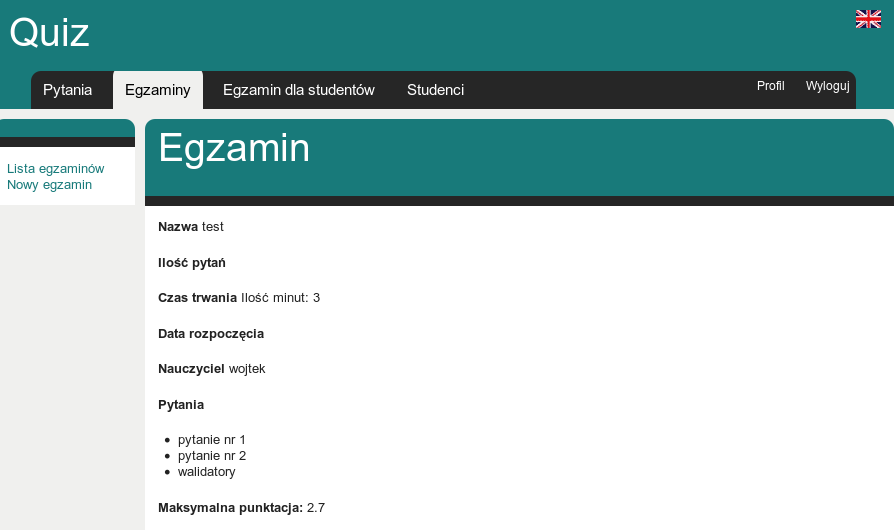
\includegraphics[width=1\linewidth]{images/layout.png}
  \end{center}
  \caption{Zrzut ekranu aplikacji}
  \label{fig:layout}
\end{figure}

\section{Wykorzystane gemy}
\subsection{Authlogic}\label{sec:authlogic}
Autorem gema \emph{Authlogic} jest Ben Johnson. Służy on jako system autentykacji,
począwszy od mechanizmu rejestracji, poprzez zarządzanie sesją użytkownika, aż do
zabezpieczeń przed próbami włamania na konto za pomocą tzw. \emph{Brute
Force}\footnote{Brute Force (ang.) -- próba złamania hasła poprzez sukcesywne sprawdzanie
wszystkich dostępnych możliwości}.


Przy tworzeniu tabeli użytkowników jest zalecane umieszczenie kilku dodatkowych kolumn,
które automatycznie się aktualizują i będą przechowywać takie informacje jak: ilość
logowań, ostatni czas aktywności, ostatni adres \emph{IP} komputera z którego nastąpiło
logowanie, etc.\\
Hasło użytkownika przed zapisaniem do bazy danych jest łączone z tzw. ,,solą'', czyli
dodatkowym ciągiem znaków, zapisywanych również w bazie danych, a następnie przeliczane
funkcją skrótu \emph{SHA1}\footnote{SHA -- Secure Hash Algorithm (ang.)}
dziesięciokrotnie, co ma utrudnić odszyfrowanie hasła z postaci samego skrótu.\\
Gem ten również zapewnia nam wszystkie niezbędne walidacje, takie jak poprawność składni
wprowadzanego adresu e-mailowego oraz loginu, zgodność hasła z potwierdzeniem, czy
unikalność istotnych atrybutów. Przykład użycia na listingu nr~\ref{listing:authlogic}.

\begin{listing}
  \input{listing/authlogic}
  \listingcaption{Sposób użycia systemu autentykacji}
  \label{listing:authlogic}
\end{listing}


W aplikacji sesja nauczyciela i studenta jest zrealizowana za pomocą jednego modelu, co
oznacza, że nie ma rozróżnienia pomiędzy sposobem logowania do serwisu. Po zalogowaniu
jednak, jest rozpoznawany typ użytkownika i na tej podstawie jest wyświetlany panel z menu
dla odpowiedniej osoby oraz sprawdzane są prawa dostępu do poszczególnych podstron.

\subsection{Acts as list}\label{sec:acts_as_list}
\emph{Acts as list} umożliwia nam dołączenie do modelu funkcjonalność listy, czyli
usystematyzowanie kolejności występowania poszczególnych rekordów. Idea ta została
wykorzystana w aplikacji przy tworzeniu pytań i dostępnych odpowiedzi w danym teście.
Dla każdego studenta, z puli dostępnych pytań, jest losowana kolejność pojawienia się ich w
teście, która jest zapisywana w bazie danych. Dzięki temu dla każdej nowej próby podejścia
do testu, czyli również dla poszczególnych studentów, kolejność ta jest różna.
Analogicznie, przy pytaniach wielokrotnego lub jednokrotnego wyboru, jest losowana
kolejność wystąpienia odpowiedzi.

\subsection{Acts as taggable on}\label{sec:acts_as_taggable_on}
\emph{Acts as taggable on} jest gemem, który łączy w sobie kilka poprzednio utworzonych
bibliotek o podobnej funkcjonalności. Dostarcza mechanizm tagowania wybranych przez
nas rekordów. Tagi mogą być tworzone w różnym kontekście, co oznacza możliwość grupowania
ich nie tylko po tworzonych, konkretnych nazwach, ale też w ujęciu poszczególnych
atrybutów. Możliwe jest również określenie właściciela poszczególnych tagów, dzięki czemu
tworzone rekordy nie muszą być globalne, a widoczne tylko dla autora.\\
Przykład wykorzystania mechanizmu tagowania na listingu nr~\ref{listing:tagging-questions}.

\begin{listing}
  \input{listing/tagging_questions}
  \listingcaption{Sposób użycia mechanizmu tagowania}
  \label{listing:tagging-questions}
\end{listing}


W aplikacji tagowanie zostało wykorzystane w klasie \texttt{TeacherQuestion}, tak aby
każdy nauczyciel miał wygodny mechanizm określania dziedziny tworzonego przez siebie
pytania. W analogiczny sposób tagi zostały dodane do modelu \texttt{Student}, aby móc
łatwo przydzielić ich do odpowiednich grup. Na listingu nr~\ref{listing:tagging-users}
kontekstem tagowania są grupy, a właścicielem nauczyciel.

\begin{listing}
  \input{listing/tagging_users}
  \listingcaption{Mechanizm tagowania w kontekście grup}
  \label{listing:tagging-users}
\end{listing}


Jak widzimy, możemy zawęzić wyszukiwanie odpowiednich rekordów do autora tagów.\\
Gem udostępnia też metody pomocnicze przy wyświetlaniu tzw. ,,chmury tagów'' w
renderowanych widokach, które możemy stylować za pomocą klas \emph{CSS}.

\subsection{Prawn}
\emph{Prawn} jest odpowiedzialny za generowanie dokumentów w formacie
\emph{PDF}\footnote{PDF -- Portable Document Format (ang.)}. Dostarcza on prosty format
szablonu, w którym możemy zagnieżdżać kod \emph{Rubiego} jednocześnie stylując
w podstawowy sposób wygląd dokumentu. Integracja z aplikacją railsową jest zapewniona
poprzez plugin \texttt{prawnto}. Pliki zapisywane są z rozszerzeniem \texttt{.pdf.prawn},
czyli zgodnie z konwencją, pierwszy element jest żądanym formatem odpowiedzi serwera,
a drugi jest nazwą silnika generującego ostateczną postać dokumentu przesłanego do klienta.\\
Przykład szablonu znajduje się na listingu nr~\ref{listing:prawn}.

\begin{listing}
  \input{listing/prawn}
  \listingcaption{Szablon wykorzystywany przy generowaniu dokumentu PDF}
  \label{listing:prawn}
\end{listing}

\subsection{Paperclip}\label{sec:paperclip}
\emph{Paperclip} jest gemem, który obsługuje ładowanie oraz obróbkę plików wysyłanych na
serwer z poziomu użytkownika. Jest zintegrowany z biblioteką \emph{ActiveRecord}, dzięki
czemu użycie nie różni się zbytnio od dobrze znanych nam konwencji. Do działania wymaga
jedynie zainstalowanej w systemie biblioteki \emph{ImageMagick}, poprzez którą są tworzone
miniaturki czy innego rodzaju konwersje na plikach graficznych. Dostajemy również zestaw
walidatorów, które mogą określać typ przesyłanego pliku oraz jego wielkość.\\
W aplikacji gem ten został wykorzystany przy załączaniu ilustracji do pytań oraz odpowiedzi.
Sposób użycia na listingu nr~\ref{listing:paperclip}.

\begin{listing}
  \input{listing/paperclip}
  \listingcaption{Sposób wykorzystania gema Paperclip}
  \label{listing:paperclip}
\end{listing}


W podanym przykładzie model \texttt{Picture} korzysta z metody \texttt{has\_attached\_file}
dostarczonej przez \emph{Paperclipa}. Przed zapisaniem, ilustracja będzie poddana obróbce
i zgodnie z kodem, wersja oryginalna zostanie przekształcona do wielkości 250 pikseli
jeśli nie jest mniejsza oraz zostanie utworzona miniaturka o proporcjonalnych
wielkościach, nie większych niż 50 pikseli. Możemy również zdefiniować ścieżkę, pod jaką
ilustracja będzie widziana z poziomu przeglądarki oraz docelowy folder
składowania w naszej aplikacji. Walidacja zapewnia, że format przyjętego pliku będzie
ograniczony tylko do \emph{JPEG}\footnote{JPEG -- nazwa jest akronimem od nazwy komitetu,
który ustanowił ten standard -- Joint Photographic Experts Group (ang.)},
\emph{PNG}\footnote{PNG -- Portable Network Graphics (ang.)} lub \emph{GIF}\footnote{GIF --
Graphics Interchange Format (ang.)}, oraz rozmiar nie przekroczy 100 kilobajtów.

\subsection{Routing filter}
Przełączanie pomiędzy różnymi wersjami językowymi aplikacji zostało zrealizowane w taki
sposób, aby był dodawany przedrostek do adresu strony w postaci kodu używanego aktualnie
języka. Drugim sposobem implementacji mogłoby być przechowywanie informacji o języku w sesji
lub ciasteczku, przez co \emph{URL} zmieniałby się tylko w chwili przełączania, a pomiędzy
kolejnymi żądaniami zmienna ta byłaby odczytywana na podstawie przechowywanej danej.
Idąc jednak za radą oficjalnych przewodników \emph{Ruby on Rails} \cite{rails-guides},
pierwszy sposób nie burzy podstawowych założeń sieci, mianowicie chcąc przesłać odnośnik
do strony, powinien on przedstawiać dokładnie tą samą treść, dlatego informacja o języku
tłumaczenia w adresie \emph{URL} jest niezbędna.


Napotykamy jednak na problem przy definiowaniu ścieżek, które są mapowane na kontrolery i
odpowiednie akcje. Okazuje się bowiem, że musielibyśmy przy każdym wewnętrznym odsyłaczu,
mapować dodatkowo parametr odpowiedzialny za informację o języku. Z pomocą jednak
przychodzi gem \emph{Routing filter}, który pozwala na używanie powyżej opisanego
mechanizmu bez przejmowania się o konfigurację ścieżek. Działa na zasadzie przechwycenia
pełnego adresu \emph{URL} przed odwołaniem się do kontrolera, sparsowaniu go, aż w końcu
po wykonaniu logiki oraz przekierowaniu, ,,doklejeniu'' usuniętego wcześniej parametru.
Twórcą gema jest Sven Fuchs, który jest również głównym autorem modułu internacjonalizacji
w \emph{Ruby on Rails}.

\subsection{Formtastic}
\emph{Formtastic} jest narzędziem, który rozbudowuje domyślny mechanizm konstruowania
formularzy w railsach, dostarczając prostszy interfejs, na rzecz zdefiniowanej przez
autora struktury oraz klas \emph{CSS}. Biblioteka ta, na podstawie asocjacji deklarowanych
w klasach, potrafi odnaleźć odpowiednią kolekcję istniejących obiektów, przy polu wyboru
formularza. Etykiety opisujące wprowadzane dane korzystają z lokalizowanych nazw atrybutów
poszczególnych modeli. Typ wyświetlonego pola formularza jest rozpoznawany na podstawie
odpowiadającej mu kolumnie w bazie danych. Wszystko to sprawia, że zbudowanie podstawowego
formularza sprowadza się do kilku linijek kodu. Przykład na listingu
nr~\ref{listing:formtastic}.

\begin{listing}
  \input{listing/formtastic}
  \listingcaption{Wykorzystanie gema upraszczającego konstruowanie formularzy}
  \label{listing:formtastic}
\end{listing}


Tworzymy nowy egzamin, pierwszym polem jest nazwa, którą wprowadzamy poprzez wpisanie
tekstu -- domyślny sposób dla kolumn typu \emph{String}. Następnie wpisujemy liczbę pytań,
która jednak nie jest pozycją wymaganą, przez co będzie otoczoną inną klasą \emph{CSS}.
Do daty rozpoczęcia, przekazujemy parametr, który ustala pierwszą z możliwych dat do
wyboru (w naszym przypadku jest to rok obecny). Do pola czasu trwania przekazujemy
wskazówkę, która wyświetli się pod wprowadzaną wartością, \emph{Formtastic} automatycznie
dodaje odpowiednie klasy, które możemy później wystylować w odpowiedni dla nas sposób. Na
samym końcu wybieramy pytania, które chcemy dołączyć, kolekcja jest tu przekazana
eksplicite, domyślnie byłyby wyświetlone wszystkie istniejące rekordy w bazie danych klasy
\texttt{Question}.

\subsection{State machine}\label{sec:state_machine}
Maszyna stanowa pozwala nam wprowadzić do obiektu pojęcie stanu w jakim obecnie się
znajduje oraz zdefiniować dostępne, czasem warunkowe, przejścia do innych stanów. Kolumna
w bazie danych, odpowiedzialna za tę informację, jest typu \emph{String}, przez co
zyskuje na czytelności. Tworzone metody pomocnicze są jednocześnie opisem pełnionych
funkcji. Przykładowa implementacja na listingu nr~\ref{listing:state-machine}.

\begin{listing}
  \input{listing/state_machine}
  \listingcaption{Sposób użycia maszyny stanowej}
  \label{listing:state-machine}
\end{listing}


Egzamin może znajdować się w trzech stanach: \texttt{prepared}, \texttt{started} oraz
\texttt{finished}, pomiędzy którymi możemy się przemieszczać za pomocą zdefiniowanych
przejść. Dodatkowo przy próbie przejścia \texttt{start} oraz \texttt{try\_finish}
sprawdzamy warunki, jeśli zwrócą fałsz, obiekty pozostaną w swoim poprzednim stanie.
Możemy również uruchomić dodatkową logikę za pomocą wywołań podobnych do tych dostępnych w
\emph{ActiveRecord}, tyle że opierających się na przejściach. I tak przy wystartowaniu
testu wywołujemy metodę, która ustawia aktualną datę i czas w atrybucie rekordu,
analogicznie rzecz się ma przy zakończeniu testu.\\
Przykładowa interakcja z maszyną stanową przy tak zdefiniowanej strukturze może wyglądać
jak na listingu nr~\ref{listing:state-machine-transitions}.

\begin{listing}
  \input{listing/state_machine_transitions}
  \listingcaption{Interakcja z maszyną stanową}
  \label{listing:state-machine-transitions}
\end{listing}


Schemat stanów oraz przejść między nimi znajduje się rysunku nr~\ref{fig:state_machine}.

\begin{figure}[h!t]
  \begin{center}
    \includegraphics[width=0.3\linewidth]{images/state_machine.pdf}
  \end{center}
  \caption{Maszyna stanowa egzaminu}
  \label{fig:state_machine}
\end{figure}


\section{Odległość Levenshteina}\label{sec:levenshtein}
Jednym z rodzajów tworzonego pytania jest pole tekstowe. Po wyborze tego właśnie typu, w
treści odpowiedzi wpisujemy wzorzec, który będzie porównany z odpowiedzią wpisaną przez
studenta.


Porównanie odbywa się na zasadzie przyrównywania kolejnych liter wzorca do otrzymanego
rozwiązania. Pojawia się jednak problem z tzw. ,,literówkami''. Co w przypadku gdy student
napisze dane słowo z dużej litery lub pomyli kolejność liter (często zdarzający się błąd)?
W celu rozwiązania powyższej przeszkody, przyjąłem dwa uproszczenia, mianowicie przy
porównaniu:
\begin{itemize}
  \item nie będzie brana pod uwagę wielkość liter
  \item na każde 6 liter wzorca jest możliwy jeden błąd
\end{itemize}


Do realizacji drugiego podpunktu została użyta odległość Levenshteina, która docelowo
oblicza wartość liczbową pomiędzy dwoma ciągami znaków, dzięki czemu jesteśmy w stanie
ocenić jak bardzo różnią się od siebie porównywane napisy.\\
Definicję można przedstawić w następujący sposób: \cite{levenshtein}


Odległością pomiędzy dwoma napisami jest najmniejsza liczba działań prostych,
przeprowadzających jeden napis w drugi, gdzie działaniem prostym nazwiemy:
\begin{itemize}
  \item wstawienie nowego znaku do napisu
  \item usunięcie znaku z napisu
  \item zamianę znaku w napisie na inny znak
\end{itemize}


Mając obliczoną odległość pomiędzy wzorcem a odpowiedzią, mierzymy długość wzorca i
dzielimy przez 6, jeśli wynik jest większy bądź równy od odległości, uznajemy odpowiedź
za poprawną. Liczba 6 została zaczerpnięta z polskiej wersji portalu NerdQuiz \cite{nerdquiz},
gdzie zastosowany jest podobny mechanizm oceny. Autorem kodu implementującego algorytm jest
Erik Veenstra \cite{veenstra}. Został on jednak przystosowany do polskich znaków oraz
problemów z kodowaniem w różnych wersjach \emph{Rubiego}\footnote{Problem został dokładniej
omówiony na stronie~\pageref{sec:ruby-versions}}. Aktualny kod znajduje się w pliku
\texttt{lib/levenshtein.rb}.

\section{Różnice pomiędzy wersjami Rubiego}\label{sec:ruby-versions}
Na dzień dzisiejszy najbardziej popularnymi wersjami języka \emph{Ruby} są:

\begin{itemize}
  \item{1.8.6}
  \item{1.8.7}
  \item{1.9.1}
\end{itemize}


Pierwsza z nich powoli wychodzi z użytku. Migracja do wersji 1.8.7 nie powinna sprawiać
problemu, gdyż jest kompatybilna wstecz. Oprócz poprawienia błędów, zostało dodanych wiele
metod, które były już dostępne w gałęzi 1.9. Autorzy chcieli potraktować tę wersję jako
przejściową, jednak znaczna większość deweloperów nie zdecydowała się na wdrożenie swoich
aplikacji przy użyciu wersji 1.9. Głównym powodem jest zmiana obsługi kodowania znaków i
problemy wynikające z tego faktu.


We wcześniejszych wersjach łańcuchy znaków były po prostu
ciągiem bajtów, przez co np. polskie litery były traktowane jako ,,dłuższe'' niż
standardowe mieszczące się w kodzie \emph{ASCII}\footnote{ASCII -- American Standard Code
for Information Interchange (ang.) -- 7-bitowy kod reprezentujący litery z alfabetu
angielskiego, cyfry, znaki przestankowe oraz kilka symboli}. Naturalnie powodowało to wiele
niedogodności, framework \emph{Ruby on Rails} wprowadził własne metody, które eliminowały
ten problem, jednak nadal trzeba było pamiętać o używaniu ich eksplicite. Biblioteka
\emph{ActiveSupport} dostarcza \texttt{mb\_chars}, która wywołana na obiekcie typu
\texttt{String}, zwraca jego reprezentację w \emph{Unikodzie}\footnote{Unicode --
zestaw znaków, który w założeniu ma obejmować wszystkie dostępne pisma na świecie}. W
wersji 1.9 wszystkie znaki są interpretowane natywnie, dlatego znikają problemy związane z
ilością bajtów w jakiej jest zapisany dany znak, jednak pojawiają się nowe, dotyczące
ustawiania odpowiedniego kodowania. Listing nr~\ref{listing:mb-chars} przedstawia
wynik operacji na różnych wersjach języka \emph{Ruby}.

\begin{listing}
  \input{listing/mb_chars}
  \listingcaption{Kodowanie znaków w różnych wersjach języka Ruby}
  \label{listing:mb-chars}
\end{listing}


Wczytując plik ze skryptem, możemy ustawić kodowanie poprzez umieszczenie w pierwszych
liniach informacji w postaci znanej np. z edytorów \emph{Emacs} lub \emph{VIM}. Wtedy
wszelkie ciągi znaków będą interpretowane tak jak sobie tego zażyczyliśmy. Wszystko to
jest możliwe poprzez klasę \emph{Encoding}, określającą sposób w jaki mają być
odczytywane bajty, w których jest zapisany dany znak. Klasa ta zawiera wiele metod, dzięki
którym jesteśmy w stanie między innymi forsować kodowanie lub sprawdzać czy dane znaki zawierają się w
\emph{ASCII}. Więcej na ten temat można znaleźć na blogu Radosława Bułata, który opisuje
również inne zmiany wprowadzone do wersji 1.9 \cite{radarek}.


Problemy jakie wynikają przy migracji do wersji 1.9 to częsta niekompatybilność gemów,
które nie są przygotowane na obsługę pełnego kodowania. Również \emph{Ruby on Rails} nie
jest wolny od tych pułapek. Domyślnie wszystkie szablony oraz przesyłane parametry są
kodowane poprzez \emph{ASCII-8BIT}. W momencie dołączenia do aplikacji plików z polskim
tłumaczeniem (\emph{UTF-8}), zwracane są wyjątki dotyczące niekompatybilności pomiędzy
oboma standardami. Niezbyt eleganckim rozwiązaniem, jednak na chwilę obecną jedynym z możliwych,
jest forsowanie kodowania do przyjętego we frameworku, poprzez tzw.
\emph{monkey patching}\footnote{Monkey patch -- znany w dynamicznych językach sposób na
rozszerzenie lub modyfikację klas o metody bez zmiany kodu źródłowego}.


W języku \emph{Ruby} jest to szczególnie proste dzięki otwartym klasom. Również w ten
sposób został rozwiązany problem uruchomienia aplikacji na wersji 1.8.6, która nie
posiada kilku metod używanych w kodzie. Listing nr~\ref{listing:monkey-patching}
przedstawia rozszerzenie klasy \emph{Array} o metodę \texttt{shuffle} w przypadku gdy nie
jest ona zdefiniowana w bibliotece standardowej.

\begin{listing}
  \input{listing/monkey_patching}
  \listingcaption{Monkey patching umożliwiający uruchomienie aplikacji na wersji 1.8.6 języka Ruby}
  \label{listing:monkey-patching}
\end{listing}


Aplikację można uruchomić na wszystkich trzech, wspomnianych wcześniej, wersjach języka
\emph{Ruby}. Wszelkie niekompatybilności zostały poprawione, tak aby nie uzależniać się od
jednego środowiska uruchomieniowego. Możemy sprawdzić to w bardzo prosty sposób.
Wystarczy, że zainstalujemy gem \emph{rvm}\footnote{RVM -- Ruby Version Manager (ang.) --
więcej na stronie \cite{rvm}}, poprzez który w prosty sposób możemy się przełączać
pomiędzy poszczególnymi wersjami. Skrypt instalacyjny mógłby wyglądać jak na listingu
nr~\ref{listing:rvm}.

\begin{listing}
  \input{listing/rvm}
  \listingcaption{Instalacja gema rvm}
  \label{listing:rvm}
\end{listing}


W chwili przełączenia jest ściągany i kompilowany kod źródłowy pożądanej wersji.
Instalowany jest on do katalogu domowego, a każda wersja posiada swój zestaw gemów.

\cleardoublepage
\chapter{Podsumowanie}
W dzisiejszych czasach na popularności zyskują projekty tworzone na otwartych licencjach,
gdzie każdy może wnieść coś od siebie do istniejącego kodu. Główną siłą takiego
podejścia jest zaangażowanie społeczności, która przecież jest końcowym odbiorcą, w
poprawę jakości oraz rozwój nowych funkcji. Zawsze też mamy możliwość modyfikacji i
dostosowania kodu do swoich indywidualnych potrzeb, co sprawia że wszelkie dostępne
narzędzia stają się niezwykle elastyczne. Przykładem na dzień dzisiejszy, potwierdzającym
powyższe rozważania, niech będzie statystyka udostępniona przez portal
\emph{Gemcutter}\footnote{Gemcutter -- od 25 października 2009 roku oficjalny hosting gemów,
dostępny również pod adresem \url{http://rubygems.org}} \cite{gemcutter}, która mówi o
7016 ogólnodostępnych gemach.


Niniejsza praca również została stworzona na otwartej licencji.
Repozytorium z kodem aplikacji znajduje się na wspominanym już wcześniej
GitHubie\footnote{Adres repozytorium to \url{http://github.com/morgoth/quiz}} i jest dostępne
publicznie. Licencja \emph{GNU GPL} nie tylko pozwala, ale wręcz zachęca do współpracy,
dlatego wszelkie wniesione poprawki i rozwinięcia będą mile widziane.


Zgodnie z założeniami, aplikacja skupia się wyłącznie na możliwości tworzenia egzaminów
internetowych przez nauczycieli oraz rozwiązywaniu ich przez uczniów, co znacznie
przyspiesza i ułatwia pracę w porównaniu do systemów typu \emph{Moodle}, gdzie trzeba
przebrnąć przez dziesiątki odsyłaczy, aby przygotować egzamin. Interfejs służący do
nawigacji po stronie jest intuicyjny i zrozumiały dla nowego użytkownika.


Kod aplikacji jest utrzymany w konwencjach przyjętych we frameworku \emph{Ruby on Rails},
dzięki czemu zrozumienie go i ewentualny przyszły rozwój przez innych programistów nie
powinien być trudny. Wszystkie modele, odpowiedzialne za główną logikę aplikacji, są pokryte
testami jednostkowymi, co przy obecnych standardach jest fundamentem każdego projektu.
Dodatkowo, najważniejsze funkcje są testowane za pomocą tzw. testów integracyjnych, które
zapewniają spójność i poprawną współpracę poszczególnych elementów.
Szata graficzna wykorzystuje ideę siatek -- strona jest podzielona na równe kolumny, które
wyznaczają obszar funkcyjny poszczególnych elementów. Wszelkie wyrównania i marginesy są
dostosowywane względem zadanej siatki, przez co zyskują na estetyce oraz standaryzują
rozmieszczenie głównych komponentów.
Wszystko to sprawia, że aplikacja jest gotowa do uruchomienia w wymiarze produkcyjnym.

\cleardoublepage
\listoflisting

\newpage
\listoffigures
\listoftables

\newpage
\bibliographystyle{plain}
\bibliography{bibliografia}
\end{document}
